\chapter[$\zmod{2}$ Homology]{Simplicial $\ZZ_2$-Homology: Physical Algebra}
\section{Intro}
This chapter, we'll talk about \emph{homology}, which captures holes in a much
more satisfying way than higher homotopy groups do.
\begin{adjustwidth}{1.5em}{}
  \begin{remark}
    Although not exactly accurate, a good way to start to understand homology for
    a space $X$ is to view an $n$-manifold in $X$ that is not the boundary of an
    $(n+1)$-manifold-with-boundary as capturing some geometry of $X$ while an
    $n$-manifold that is the boundary of an $(n+1)$-dimensional
    manifold-with-boundary is not detecting any hole or structure.
  \end{remark}
\end{adjustwidth}
\section{Chains, Cycles, Boundaries, and the Homology Groups}
\begin{definition}[$n$-chain]
  An \emph{$n$-chain} of $K$ is a finite formal sum
  \[
    \sum_{i=1}^k \sigma_i
  \]
  of distinct $n$-simplices in $K$. Note that the dimensions of the simplices
  must be the same. So \emph{chain} will mean $n$-chain whenever the dimension
  is either unimportant or understood.
\end{definition}
\begin{definition}[$n$-chain group]
  The \emph{$n$-chain group of $K$} (with coefficients in $\zmod{2}$), denoted
  $\mathsf{C}_n(K)$, is the collection of $n$-chains in $K$ under formal
  addition modulo 2. If there are no $n$-simplices in $K$, the $n$-chain group
  of $K$ is defined to be trivial (containing the ``empty'' chain).
\end{definition}
\begin{problem}[16.1]
  Check that $\msf C_n(K)$ is an abelian group.
\end{problem}
\begin{solution}
  \begin{enumerate}[label=(\arabic*)]
  \item $\epsilon = \sum_{i \in \varnothing} \sigma_i$.
  \item Associativity inherited from $\cup$.
  \item Closure inherited from $\cup$ over the domain given.
  \item Existence of inverses --- since we're taking formal linear
    combinations over $\zmod{2}$, then every element is its own inverse.
  \end{enumerate}
  Finally, to see that $\msf C_n(K)$ is abelian, observe that $+$ in $\msf
  C_n(K)$ inherits commutativity from $\cup$.
\end{solution}
\begin{definition}[$\zmod{2}$ boundary of a simplex]
  The \emph{$\zmod{2}$-boundary of an $n$-simplex $\sigma = \simp{n}$} is
  defined by
  \[
    \partial \sigma = \sum_{i=0}^n \simpdel{i}{n}
  \]
  the formal sum of the $(n-1)$-faces of $\sigma$.

  For a 0-simplex, the $\zmod{2}$ boundary is defined to be $0 \in \msf
  C_{-1}(K)$.
\end{definition}
\begin{definition}[$\zmod{2}$ boundary of an $n$-chain]
  The \emph{$\zmod{2}$ boundary of an $n$-chain} is the sum of the boundaries of
  the simplices. That is, $\partial_n : \msf C_n(K) \to \msf C_{n-1}(K)$ is
  given by
  \[
    \partial\pn{\sum_{i=1}^k \sigma_i} = \sum_{i=1}^k \partial(\sigma_i)
  \]
\end{definition}
\begin{problem}[16.2]
  Verify that $\partial$ is a homomorphism, and use the definition to compute
  the $\zmod{2}$ boundary of $\sigma_1 + \sigma_2$ in Figure 16.1
\end{problem}
\begin{solution}
  We want to show $\partial$ is a homomorphism.
  \begin{enumerate}
  \item Let $\epsilon_n \in \msf C_n(K)$ be identity. We want to show
    $\partial(\epsilon_n) = \epsilon_{n-1}$. Taking the empty sum to be
    identity, we see
    \begin{align*}
      \partial(\epsilon_n)
      &=
        \partial\pn{\sum_{i\in \varnothing} \sigma_i} \\
      &= \sum_{i\in\varnothing} \partial\pn{\sigma_i} \\
      &= \epsilon_{n-1}
    \end{align*}
    as desired.
  \item That $\partial$ respects addition is definitional.
  \end{enumerate}
  We have $\partial(\sigma_1 + \sigma_2) = e_1 + e_2 + e_4 + e_5$.
\end{solution}
\begin{definition}[$n$-cycle and $n$-boundary]
  An \emph{$n$-cycle} is an $n$-chain of $K$ whose boundary is zero. The set of
  all $n$-cycles on $K$ is denoted $\msf Z_n(K)$. An \emph{$n$-boundary} is an
  $n$-chain that is the boundary of an $(n+1)$-chain of $K$. The set of all
  $n$-boundaries is denoted $\msf B_n(K)$.
\end{definition}
% \begin{problem}[16.3]

% \end{problem}
\begin{problem}[16.4]
  Both $\msf Z_n(K)$ and $\msf B_n(K)$ are subgroups of $\msf C_n(K)$. Moreover,
  \[
    \partial \circ \partial = 0.
  \]
  In other words, $\partial_n \circ \partial_{n+1} = 0$ for each index $n \geq
  0$. Hence, $\msf B_n(K) \subset \msf Z_n(K)$.
\end{problem}
\begin{solution}
  Let $\sigma_1, \sigma_2 \in \msf Z_n(K)$. Then by linearity of $\partial_n$,
  we have
  \begin{align*}
    \partial_n(\sigma_1 + \sigma_2)
    &= \partial_n(\sigma_1) + \partial_n(\sigma_2) \\
    &= 0
  \end{align*}
  and hence $\msf Z_n(K) < \msf C_n(K)$.

  Now, let $\sigma_1, \sigma_2 \in \msf B_n(K)$. Then $\exists \tau_1, \tau_2
  \in \msf Z_{n+1}(K)$ such that $\partial_{n+1}(\tau_1) = \sigma_1,
  \partial_{n+1}(\tau_2) = \sigma_{2}$. Since $\msf Z_{n+1}(K) < \msf
  C_{n+1}(K)$, then $\tau_1 + \tau_2 \in \msf Z_{n+1}(K)$. Now, by linearity of
  $\partial$, we have
  \begin{align*}
    \partial_{n+1}(\tau_1 + \tau_2)
    &= \partial_{n+1}(\tau_1) + \partial_{n+1}(\tau_2) \\
    &= \sigma_1 + \sigma_2
  \end{align*}
  hence $\msf B_n(K)$ is a subset closed under the operation, so we have $\msf
  B_n(K) < \msf C_n(K)$.

  It remains to show $\partial_n \circ \partial_{n+1} = 0$. Let $\sigma \in \msf
  C_{n+1}(K)$. Then
  \begin{align*}
    \partial_{n+1}(\sigma)
    &= \partial_{n+1}\pn{\sum_{i \in I} \simp[v^{(i)}]{n+1}} \\
    &= \sum_{i\in I} \partial_{n+1}\pn{\simp[v^{(i)}]{n+1}} \\
    &= \sum_{i\in I} \sum_{j \in [n+1]} \simpdel[v^{(i)}]{j}{n+1}
  \end{align*}
  and so
  \begin{align*}
    \partial_n \pn{\partial_{n+1}(\sigma)}
    &= \sum_{i\in I} \sum_{j \in [n+1]} \partial_{n}\pn{\simpdel[v^{(i)}]{j}{n+1}} \\
    &= \sum_{i\in I} \sum_{j \in [n+1]} \sum_{\substack{k \in [n+1] \\ k \neq j}} \set{v_0^{(i)} \cdots \widehat{v_k^{(i)}} \cdots \widehat{v_j^{(i)}}\cdots v^{(i)}_{n+1}}
  \end{align*}
  hence all the terms cancel, and we're left with $\mb 0$. So $\partial_n \circ
  \partial_{n+1} = 0$, as desired.

  Since every $\sigma \in \msf B_n(K)$ is of the form $\partial_{n+1}(\tau)$
  where $\tau \in \msf C_{n+1}(K)$, it follows that $\partial_n\fim[\msf
  B_n(K)] = (\partial_n \circ \partial_{n+1}) (\msf C_{n+1}(K)) = 0$. Thus $\msf
  B_n(K) < \msf Z_n(K)$.
\end{solution}
\begin{definition}[Homologous cycles]
  Two $n$-cycles $\alpha$ and $\beta$ in $K$ are \emph{equivalent} or
  \emph{homologous} iff $\alpha-\beta = \partial(\gamma)$ for some $(n+1)$-chain
  $\gamma$. In other words, $\alpha$ and $\beta$ are homologous iff they differ
  by an element of the subgroup $\msf B_n(K)$, denoted by
  \[
    \alpha \sim_{\zmod{2}} \beta.
  \]
  The equivalence class of $\alpha$ is denoted by enclosing it in brackets
  thusly: $[\alpha]$. For $\zmod{2}$ $n$-chains, observe that $\alpha - \beta =
  \alpha + \beta$. So we see that two $n$-cycles are equivalent if together they
  bound an $(n+1)$-chain.
\end{definition}
\begin{definition}[$n$\textsuperscript{th} Homology group]
  The \emph{$n$\textsuperscript{th}-homology group} (with coefficients in
  $\zmod{2}$) of a finite simplicial complex $K$, denoted $\msf H_n(K)$, is the
  additive group whose elements are equivalence classes of cycles under the
  $\zmod{2}$-equivalence defined above, with $\bk{\alpha} + \bk{\beta} =
  \bk{\alpha +\beta}$. I.e.,
  \[
    \msf H_n(K) = \msf Z_n(K)/\msf B_n(K)
  \]
\end{definition}
\begin{problem}[F1]
  Consider the simplicial complex given below in Figure \cref{fig:FK1}. Then for
  $n = 0, 1, 2$,
  \begin{enumerate}
  \item describe elements of $\msf C_n(K)$,
  \item compute $\msf Z_n(K)$,
  \item compute $\msf B_n(K)$, and
  \item compute $\msf H_n(K)$.
  \end{enumerate}
\end{problem}
\begin{figure}[H]
  \centering
  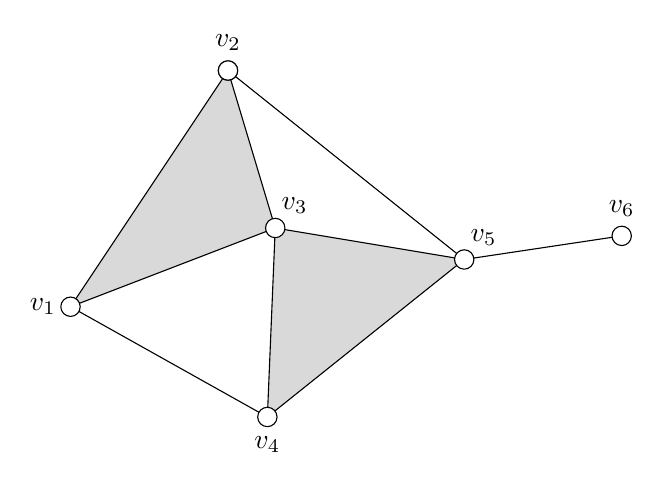
\begin{tikzpicture}[
    every node/.style={
      circle,
      draw=black,
      fill=white,
      inner sep=0pt,
      minimum size=7pt
    }
    ]

    \coordinate (v1) at (0,0);
    \coordinate (v2) at (2,3);
    \coordinate (v3) at (2.6,1);
    \coordinate (v4) at (2.5,-1.4);
    \coordinate (v5) at (5,.6);
    \coordinate (v6) at (7,.9);

    \draw[fill=gray!30!white] (v1) -- (v2) -- (v3) -- (v1) -- cycle;
    \draw[fill=gray!30!white] (v3) -- (v4) -- (v5) -- (v3) -- cycle;

    \draw (v1) -- (v4);
    \draw (v2) -- (v5);
    \draw (v5) -- (v6);

    \node (wv1) at (v1) {};
    \node (wv2) at (v2) {};
    \node (vv2) at (v2) {};
    \node (vv3) at (v3) {};
    \node (vv4) at (v4) {};
    \node (vv5) at (v5) {};
    \node (vv6) at (v6) {};

    \node[draw=none, xshift=-1em] (wv1) at (v1) {$v_1$};
    \node[draw=none, yshift=1em] (wv2) at (v2) {$v_2$};
    \node[draw=none, xshift=.7em, yshift=.8em] (wv3) at (v3) {$v_3$};
    \node[draw=none, yshift=-1em] (wv4) at (v4) {$v_4$};
    \node[draw=none, xshift=.7em, yshift=.8em] (wv5) at (v5) {$v_5$};
    \node[draw=none, yshift=1em] (wv6) at (v6) {$v_6$};
  \end{tikzpicture}
  \caption{Simplicial complex $K$}
  \label{fig:F1}
\end{figure}
\begin{solution}
  First, we redraw the simplicial complex as follows:
  \begin{figure}[H]
    \centering
    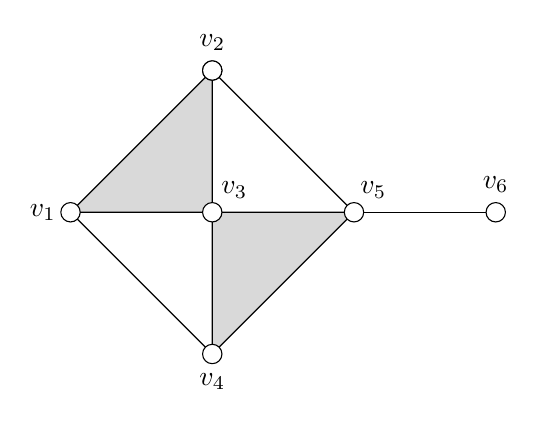
\begin{tikzpicture}[
      scale = .6,
      every node/.style={
        circle,
        draw=black,
        fill=white,
        inner sep=0pt,
        minimum size=7pt
      }
      ]

      \coordinate (v1) at (-3,0);
      \coordinate (v2) at (0,3);
      \coordinate (v3) at (0,0);
      \coordinate (v4) at (0,-3);
      \coordinate (v5) at (3,0);
      \coordinate (v6) at (6,0);

      \draw[fill=gray!30!white] (v1) -- (v2) -- (v3) -- (v1) -- cycle;
      \draw[fill=gray!30!white] (v3) -- (v4) -- (v5) -- (v3) -- cycle;

      \draw (v1) -- (v4);
      \draw (v2) -- (v5);
      \draw (v5) -- (v6);

      \node (wv1) at (v1) {};
      \node (wv2) at (v2) {};
      \node (vv2) at (v2) {};
      \node (vv3) at (v3) {};
      \node (vv4) at (v4) {};
      \node (vv5) at (v5) {};
      \node (vv6) at (v6) {};

      \node[draw=none, xshift=-1em] (wv1) at (v1) {$v_1$};
      \node[draw=none, yshift=1em] (wv2) at (v2) {$v_2$};
      \node[draw=none, xshift=.8em, yshift=.8em] (wv3) at (v3) {$v_3$};
      \node[draw=none, yshift=-1em] (wv4) at (v4) {$v_4$};
      \node[draw=none, xshift=.7em, yshift=.8em] (wv5) at (v5) {$v_5$};
      \node[draw=none, yshift=1em] (wv6) at (v6) {$v_6$};
    \end{tikzpicture}
    \caption{Simplicial complex $K$, straightened out}
  \end{figure}
  For the purposes of this problem, take angled brackets indicate span. We have
  \begin{enumerate}[label=(\roman*)]
  \item We calculate the $k=0$ case.
    \begin{enumerate}
    \item Elements of $\msf C_0(K)$ are formal linear combinations over the
      set $\set{v_1, v_2, \ldots, v_6}$. Then
      \[
        \msf C_0(K) = \ip[Big]{v_1, v_2, v_3, v_4, v_5, v_6}
      \]
      that is, collections of points in $\msf C_0(K)$.
    \item Let $\sigma_1, \ldots, \sigma_k \in \msf C_0(K).$ Then by definition,
      \begin{align*}
        \partial\pn{\sum_{i=1}^k \sigma_i}
        &= \sum_{i=1}^k \partial(\sigma_i)\\
        &= \sum_{i=1}^k 0 \\
        &= 0
      \end{align*}
      hence $\msf Z_n(K) = \msf C_n(K)$.
    \item A $\sigma \in \msf C_0(K)$ is an $n$-boundary if $\exists \tau \in
      \msf C_{1}(K)$ with $\partial(\tau) = \sigma$. Note, for any
      $1$-dimensional face $\set{v_iv_j} \in K$,
      \begin{align*}
        \partial(\set{v_iv_j})
        &= \set{v_i \widehat{v_j}} + \set{\widehat{v_i}v_j} \\
        &= \set{v_i} + \set{v_j} \\
        &= \delta_{ij}.
      \end{align*}
      Hence, any edge formed of a pair of two distinct vertices yields a
      nonempty boundary. We first count all edges:
      \begin{figure}[H]
        \centering
        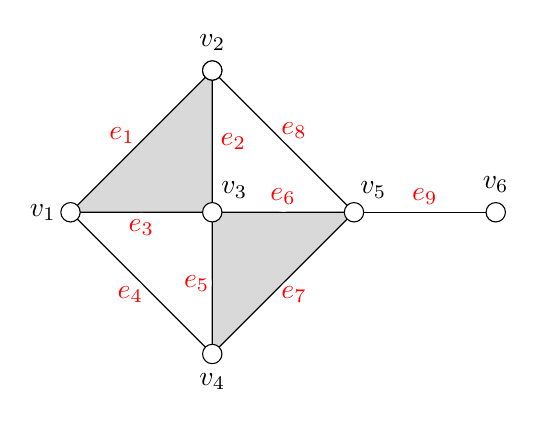
\begin{tikzpicture}[
          scale = .6,
          every node/.style={
            circle,
            draw=black,
            fill=white,
            inner sep=0pt,
            minimum size=7pt
          }
          ]

          \coordinate (v1) at (-3,0);
          \coordinate (v2) at (0,3);
          \coordinate (v3) at (0,0);
          \coordinate (v4) at (0,-3);
          \coordinate (v5) at (3,0);
          \coordinate (v6) at (6,0);

          \draw[fill=gray!30!white] (v1) -- (v2)
          % draw and label the edge between v1 and v2
          node[draw=none, midway, above left, xshift=-.3em, yshift=-.2em]
          {\color{red} $e_1$} -- (v3)
          % draw the edge between v2 and v3, and label it as well
          node[draw=none, midway, right, xshift=.2em] {\color{red} $e_2$}
          -- (v1)
          % draw the edge between v3 and v1, and label it as well
          node[draw=none, midway, below] {\color{red}$e_3$} -- cycle;

          \draw (v1) -- (v4) node[draw=none, midway, below left] {\color{red} $e_4$};

          \draw[fill=gray!30!white] (v3) -- (v4)
          % edge between v3 and and v4
          node[draw=none, midway, left] {\color{red} $e_5$} -- (v5)
          % edge
          node[draw=none, midway, below right] {\color{red}$e_7$} -- (v3)
          %
          node[draw=none, midway, above] {\color{red} $e_6$} -- cycle;


          \draw (v2) -- (v5) node[draw=none, midway, above right] {\color{red} $e_8$};
          \draw (v5) -- (v6) node[draw=none, midway, above] {\color{red} $e_9$};

          \node (wv1) at (v1) {};
          \node (wv2) at (v2) {};
          \node (vv2) at (v2) {};
          \node (vv3) at (v3) {};
          \node (vv4) at (v4) {};
          \node (vv5) at (v5) {};
          \node (vv6) at (v6) {};

          \node[draw=none, xshift=-1em] (wv1) at (v1) {$v_1$};
          \node[draw=none, yshift=1em] (wv2) at (v2) {$v_2$};
          \node[draw=none, xshift=.8em, yshift=.8em] (wv3) at (v3) {$v_3$};
          \node[draw=none, yshift=-1em] (wv4) at (v4) {$v_4$};
          \node[draw=none, xshift=.7em, yshift=.8em] (wv5) at (v5) {$v_5$};
          \node[draw=none, yshift=1em] (wv6) at (v6) {$v_6$};
        \end{tikzpicture}
        \caption{Simplicial complex $K$ with simple edges}
      \end{figure}
      Since $\msf B_0(K)$ is a subgroup of $\msf C_0(K)$, by closure under
      $+$, we see that any $v_i+v_j$ in $K$ such that there exists a path
      from $v_i$ to $v_j$ (when $K$ is considered a graph) is an element of
      $\msf B_0(K)$. In fact, we can say more:

      \textbf{Claim:} Since $K$ is connected as a graph, any even collection
      of vertices is in $\msf B_n(K)$.

      \textbf{Proof of Claim:} Suppose we have $\sigma = \set{v_{i_1}} +
      \set{v_{i_2}} + \cdots + \set{v_{i_{2k}}}$, where $k \in \NN$. Then
      for each $j = 1, \ldots, k$, let $\tau_j$ be a sum of edges representing
      a path from $v_{i_j}$ to $v_{i_{j+1}}$. For example, if $v_{i_j} =
      v_6$ and $v_{i_{j+1}} = v_2$, we could take the following approaches:
      \begin{figure}[H]
        \centering
        \begin{subfigure}{.49\linewidth}
          \centering
          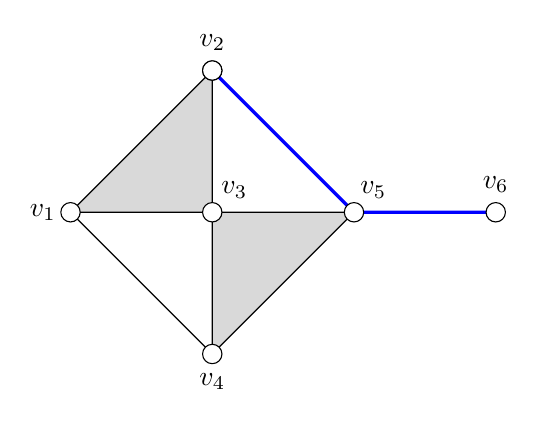
\begin{tikzpicture}[
            scale = .6,
            every node/.style={
              circle,
              draw=black,
              fill=white,
              inner sep=0pt,
              minimum size=7pt
            }
            ]

            \coordinate (v1) at (-3,0);
            \coordinate (v2) at (0,3);
            \coordinate (v3) at (0,0);
            \coordinate (v4) at (0,-3);
            \coordinate (v5) at (3,0);
            \coordinate (v6) at (6,0);

            \draw[fill=gray!30!white] (v1) -- (v2) -- (v3) -- (v1) -- cycle;
            \draw[fill=gray!30!white] (v3) -- (v4) -- (v5) -- (v3) -- cycle;

            \draw (v1) -- (v4);
            \draw (v2) -- (v5);
            \draw (v5) -- (v6);

            \draw[draw=blue, very thick] (v6) -- (v5) -- (v2);

            \node (wv1) at (v1) {};
            \node (wv2) at (v2) {};
            \node (vv2) at (v2) {};
            \node (vv3) at (v3) {};
            \node (vv4) at (v4) {};
            \node (vv5) at (v5) {};
            \node (vv6) at (v6) {};

            \node[draw=none, xshift=-1em] (wv1) at (v1) {$v_1$};
            \node[draw=none, yshift=1em] (wv2) at (v2) {$v_2$};
            \node[draw=none, xshift=.8em, yshift=.8em] (wv3) at (v3) {$v_3$};
            \node[draw=none, yshift=-1em] (wv4) at (v4) {$v_4$};
            \node[draw=none, xshift=.7em, yshift=.8em] (wv5) at (v5) {$v_5$};
            \node[draw=none, yshift=1em] (wv6) at (v6) {$v_6$};
          \end{tikzpicture}
        \end{subfigure}
        \begin{subfigure}{.49\linewidth}
          \centering
          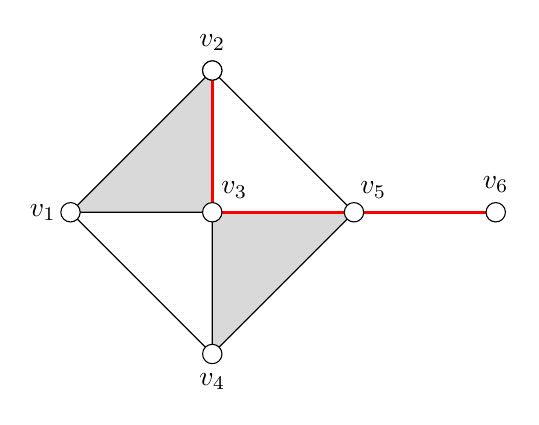
\begin{tikzpicture}[
            scale = .6,
            every node/.style={
              circle,
              draw=black,
              fill=white,
              inner sep=0pt,
              minimum size=7pt
            }
            ]

            \coordinate (v1) at (-3,0);
            \coordinate (v2) at (0,3);
            \coordinate (v3) at (0,0);
            \coordinate (v4) at (0,-3);
            \coordinate (v5) at (3,0);
            \coordinate (v6) at (6,0);

            \draw[fill=gray!30!white] (v1) -- (v2) -- (v3) -- (v1) -- cycle;
            \draw[fill=gray!30!white] (v3) -- (v4) -- (v5) -- (v3) -- cycle;

            \draw (v1) -- (v4);
            \draw (v2) -- (v5);
            \draw (v5) -- (v6);

            \draw[draw=red, very thick] (v6) -- (v5) -- (v3) -- (v2);

            \node (wv1) at (v1) {};
            \node (wv2) at (v2) {};
            \node (vv2) at (v2) {};
            \node (vv3) at (v3) {};
            \node (vv4) at (v4) {};
            \node (vv5) at (v5) {};
            \node (vv6) at (v6) {};

            \node[draw=none, xshift=-1em] (wv1) at (v1) {$v_1$};
            \node[draw=none, yshift=1em] (wv2) at (v2) {$v_2$};
            \node[draw=none, xshift=.8em, yshift=.8em] (wv3) at (v3) {$v_3$};
            \node[draw=none, yshift=-1em] (wv4) at (v4) {$v_4$};
            \node[draw=none, xshift=.7em, yshift=.8em] (wv5) at (v5) {$v_5$};
            \node[draw=none, yshift=1em] (wv6) at (v6) {$v_6$};
          \end{tikzpicture}
        \end{subfigure}
        \begin{subfigure}{.49\linewidth}
          \centering
          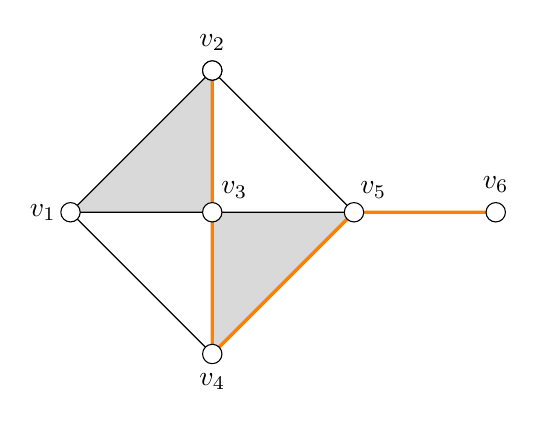
\begin{tikzpicture}[
            scale = .6,
            every node/.style={
              circle,
              draw=black,
              fill=white,
              inner sep=0pt,
              minimum size=7pt
            }
            ]

            \coordinate (v1) at (-3,0);
            \coordinate (v2) at (0,3);
            \coordinate (v3) at (0,0);
            \coordinate (v4) at (0,-3);
            \coordinate (v5) at (3,0);
            \coordinate (v6) at (6,0);

            \draw[fill=gray!30!white] (v1) -- (v2) -- (v3) -- (v1) -- cycle;
            \draw[fill=gray!30!white] (v3) -- (v4) -- (v5) -- (v3) -- cycle;

            \draw (v1) -- (v4);
            \draw (v2) -- (v5);
            \draw (v5) -- (v6);

            \draw[draw=orange, very thick] (v6) -- (v5) -- (v4) -- (v3)-- (v2);

            \node (wv1) at (v1) {};
            \node (wv2) at (v2) {};
            \node (vv2) at (v2) {};
            \node (vv3) at (v3) {};
            \node (vv4) at (v4) {};
            \node (vv5) at (v5) {};
            \node (vv6) at (v6) {};

            \node[draw=none, xshift=-1em] (wv1) at (v1) {$v_1$};
            \node[draw=none, yshift=1em] (wv2) at (v2) {$v_2$};
            \node[draw=none, xshift=.8em, yshift=.8em] (wv3) at (v3) {$v_3$};
            \node[draw=none, yshift=-1em] (wv4) at (v4) {$v_4$};
            \node[draw=none, xshift=.7em, yshift=.8em] (wv5) at (v5) {$v_5$};
            \node[draw=none, yshift=1em] (wv6) at (v6) {$v_6$};
          \end{tikzpicture}
        \end{subfigure}
        \begin{subfigure}{.49\linewidth}
          \centering
          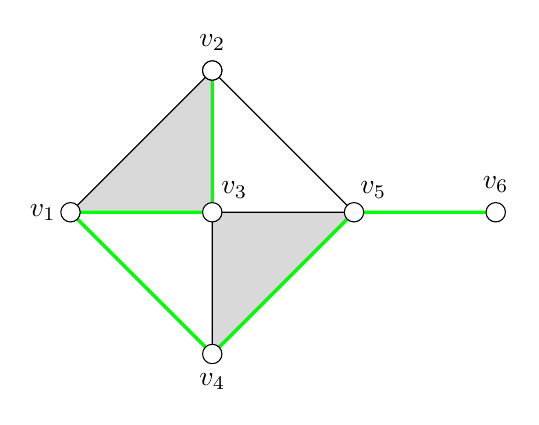
\begin{tikzpicture}[
            scale = .6,
            every node/.style={
              circle,
              draw=black,
              fill=white,
              inner sep=0pt,
              minimum size=7pt
            }
            ]

            \coordinate (v1) at (-3,0);
            \coordinate (v2) at (0,3);
            \coordinate (v3) at (0,0);
            \coordinate (v4) at (0,-3);
            \coordinate (v5) at (3,0);
            \coordinate (v6) at (6,0);

            \draw[fill=gray!30!white] (v1) -- (v2) -- (v3) -- (v1) -- cycle;
            \draw[fill=gray!30!white] (v3) -- (v4) -- (v5) -- (v3) -- cycle;

            \draw (v1) -- (v4);
            \draw (v2) -- (v5);
            \draw (v5) -- (v6);

            \draw[draw=green, very thick] (v6) -- (v5) -- (v4) -- (v1) -- (v3) -- (v2);

            \node (wv1) at (v1) {};
            \node (wv2) at (v2) {};
            \node (vv2) at (v2) {};
            \node (vv3) at (v3) {};
            \node (vv4) at (v4) {};
            \node (vv5) at (v5) {};
            \node (vv6) at (v6) {};

            \node[draw=none, xshift=-1em] (wv1) at (v1) {$v_1$};
            \node[draw=none, yshift=1em] (wv2) at (v2) {$v_2$};
            \node[draw=none, xshift=.8em, yshift=.8em] (wv3) at (v3) {$v_3$};
            \node[draw=none, yshift=-1em] (wv4) at (v4) {$v_4$};
            \node[draw=none, xshift=.7em, yshift=.8em] (wv5) at (v5) {$v_5$};
            \node[draw=none, yshift=1em] (wv6) at (v6) {$v_6$};
          \end{tikzpicture}
        \end{subfigure}
      \end{figure}\clearpage
      \begin{figure}[H]\ContinuedFloat
        \begin{subfigure}{.49\linewidth}
          \centering
          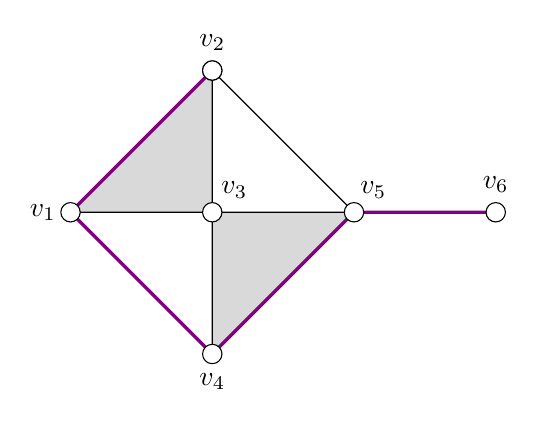
\begin{tikzpicture}[
            scale = .6,
            every node/.style={
              circle,
              draw=black,
              fill=white,
              inner sep=0pt,
              minimum size=7pt
            }
            ]

            \coordinate (v1) at (-3,0);
            \coordinate (v2) at (0,3);
            \coordinate (v3) at (0,0);
            \coordinate (v4) at (0,-3);
            \coordinate (v5) at (3,0);
            \coordinate (v6) at (6,0);

            \draw[fill=gray!30!white] (v1) -- (v2) -- (v3) -- (v1) -- cycle;
            \draw[fill=gray!30!white] (v3) -- (v4) -- (v5) -- (v3) -- cycle;

            \draw (v1) -- (v4);
            \draw (v2) -- (v5);
            \draw (v5) -- (v6);

            \draw[draw=violet, very thick] (v6) -- (v5) -- (v4) -- (v1)-- (v2);

            \node (wv1) at (v1) {};
            \node (wv2) at (v2) {};
            \node (vv2) at (v2) {};
            \node (vv3) at (v3) {};
            \node (vv4) at (v4) {};
            \node (vv5) at (v5) {};
            \node (vv6) at (v6) {};

            \node[draw=none, xshift=-1em] (wv1) at (v1) {$v_1$};
            \node[draw=none, yshift=1em] (wv2) at (v2) {$v_2$};
            \node[draw=none, xshift=.8em, yshift=.8em] (wv3) at (v3) {$v_3$};
            \node[draw=none, yshift=-1em] (wv4) at (v4) {$v_4$};
            \node[draw=none, xshift=.7em, yshift=.8em] (wv5) at (v5) {$v_5$};
            \node[draw=none, yshift=1em] (wv6) at (v6) {$v_6$};
          \end{tikzpicture}
        \end{subfigure}
        \begin{subfigure}{.49\linewidth}
          \centering
          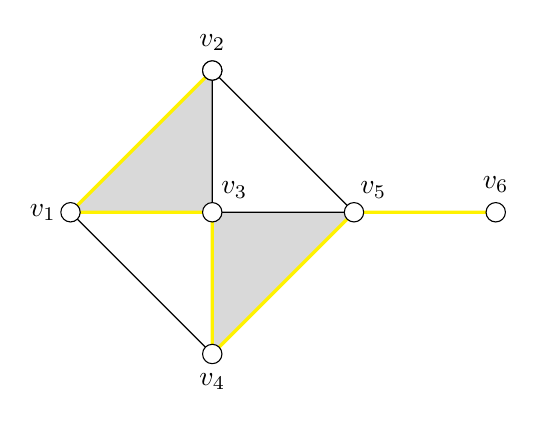
\begin{tikzpicture}[
            scale = .6,
            every node/.style={
              circle,
              draw=black,
              fill=white,
              inner sep=0pt,
              minimum size=7pt
            }
            ]

            \coordinate (v1) at (-3,0);
            \coordinate (v2) at (0,3);
            \coordinate (v3) at (0,0);
            \coordinate (v4) at (0,-3);
            \coordinate (v5) at (3,0);
            \coordinate (v6) at (6,0);

            \draw[fill=gray!30!white] (v1) -- (v2) -- (v3) -- (v1) -- cycle;
            \draw[fill=gray!30!white] (v3) -- (v4) -- (v5) -- (v3) -- cycle;

            \draw (v1) -- (v4);
            \draw (v2) -- (v5);
            \draw (v5) -- (v6);

            \draw[draw=yellow, very thick] (v6) -- (v5) -- (v4) -- (v3) -- (v1) -- (v2);

            \node (wv1) at (v1) {};
            \node (wv2) at (v2) {};
            \node (vv2) at (v2) {};
            \node (vv3) at (v3) {};
            \node (vv4) at (v4) {};
            \node (vv5) at (v5) {};
            \node (vv6) at (v6) {};

            \node[draw=none, xshift=-1em] (wv1) at (v1) {$v_1$};
            \node[draw=none, yshift=1em] (wv2) at (v2) {$v_2$};
            \node[draw=none, xshift=.8em, yshift=.8em] (wv3) at (v3) {$v_3$};
            \node[draw=none, yshift=-1em] (wv4) at (v4) {$v_4$};
            \node[draw=none, xshift=.7em, yshift=.8em] (wv5) at (v5) {$v_5$};
            \node[draw=none, yshift=1em] (wv6) at (v6) {$v_6$};
          \end{tikzpicture}
        \end{subfigure}
        \caption{Some paths from $v_6$ to $v_2$}
      \end{figure}
      among others. Taking the sum of the constituent edges in each path
      yields a sum of $1$-simplices with boundary $v_6,
      v_2$.\footnote{Justification: note that the coefficient on any given
        vertex when we apply $\partial$ is the degree of the vertex in our
        path. Hence, only the initial and terminal vertex don't get mapped
        to $0$.}
    \item Since $\msf B_n(K)$ is the group of all collections of even
      vertices in $\msf C_n(K)$, we have $\msf H_n(K) = \msf C_n(K)/\msf
      B_n(K) \cong \zmod{2}$.
    \end{enumerate}
  \item Now, we calculate the $k=1$ case.
    \begin{enumerate}
    \item Elements of $\msf C_1(K)$ are collections of linear combinations
      of the edges
      \[
        \msf C_1(K) = \ip{e_1, e_2, e_3, e_4, e_5, e_6, e_7, e_8, e_9}
      \]
    \item Elements of $\msf Z_1(K)$ are collections of edges such that
      each vertex contained in an edge in the collection has even degree.
      This corresponds to cyclic subgraphs of $K$ (as well as the empty
      cycle), e.g.:
      \begin{figure}[H]
        \centering
        \begin{subfigure}{.49\linewidth}
          \centering
          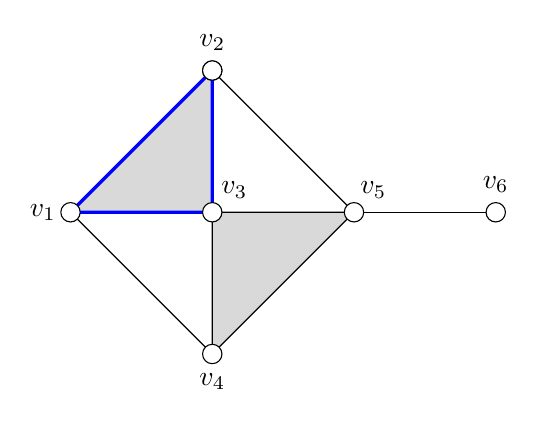
\begin{tikzpicture}[
            scale = .6,
            every node/.style={
              circle,
              draw=black,
              fill=white,
              inner sep=0pt,
              minimum size=7pt
            }
            ]

            \coordinate (v1) at (-3,0);
            \coordinate (v2) at (0,3);
            \coordinate (v3) at (0,0);
            \coordinate (v4) at (0,-3);
            \coordinate (v5) at (3,0);
            \coordinate (v6) at (6,0);

            \draw[fill=gray!30!white] (v1) -- (v2) -- (v3) -- (v1) -- cycle;
            \draw[fill=gray!30!white] (v3) -- (v4) -- (v5) -- (v3) -- cycle;

            \draw (v1) -- (v4);
            \draw (v2) -- (v5);
            \draw (v5) -- (v6);

            \draw[draw=blue, very thick] (v1) -- (v2) -- (v3) -- cycle;

            \node (wv1) at (v1) {};
            \node (wv2) at (v2) {};
            \node (vv2) at (v2) {};
            \node (vv3) at (v3) {};
            \node (vv4) at (v4) {};
            \node (vv5) at (v5) {};
            \node (vv6) at (v6) {};

            \node[draw=none, xshift=-1em] (wv1) at (v1) {$v_1$};
            \node[draw=none, yshift=1em] (wv2) at (v2) {$v_2$};
            \node[draw=none, xshift=.8em, yshift=.8em] (wv3) at (v3) {$v_3$};
            \node[draw=none, yshift=-1em] (wv4) at (v4) {$v_4$};
            \node[draw=none, xshift=.7em, yshift=.8em] (wv5) at (v5) {$v_5$};
            \node[draw=none, yshift=1em] (wv6) at (v6) {$v_6$};
          \end{tikzpicture}
        \end{subfigure}
        \begin{subfigure}{.49\linewidth}
          \centering
          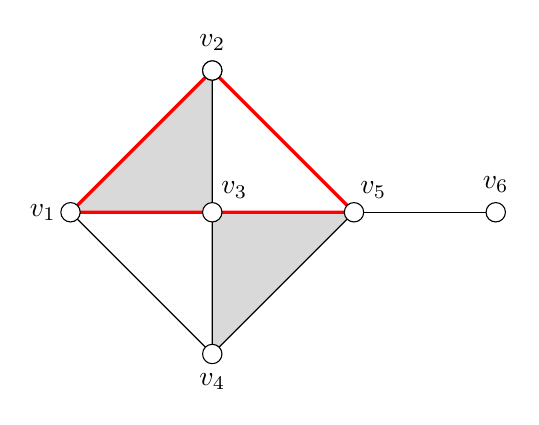
\begin{tikzpicture}[
            scale = .6,
            every node/.style={
              circle,
              draw=black,
              fill=white,
              inner sep=0pt,
              minimum size=7pt
            }
            ]

            \coordinate (v1) at (-3,0);
            \coordinate (v2) at (0,3);
            \coordinate (v3) at (0,0);
            \coordinate (v4) at (0,-3);
            \coordinate (v5) at (3,0);
            \coordinate (v6) at (6,0);

            \draw[fill=gray!30!white] (v1) -- (v2) -- (v3) -- (v1) -- cycle;
            \draw[fill=gray!30!white] (v3) -- (v4) -- (v5) -- (v3) -- cycle;

            \draw (v1) -- (v4);
            \draw (v2) -- (v5);
            \draw (v5) -- (v6);

            \draw[draw=red, very thick] (v1) -- (v2) -- (v5) -- (v3) -- (v1);

            \node (wv1) at (v1) {};
            \node (wv2) at (v2) {};
            \node (vv2) at (v2) {};
            \node (vv3) at (v3) {};
            \node (vv4) at (v4) {};
            \node (vv5) at (v5) {};
            \node (vv6) at (v6) {};

            \node[draw=none, xshift=-1em] (wv1) at (v1) {$v_1$};
            \node[draw=none, yshift=1em] (wv2) at (v2) {$v_2$};
            \node[draw=none, xshift=.8em, yshift=.8em] (wv3) at (v3) {$v_3$};
            \node[draw=none, yshift=-1em] (wv4) at (v4) {$v_4$};
            \node[draw=none, xshift=.7em, yshift=.8em] (wv5) at (v5) {$v_5$};
            \node[draw=none, yshift=1em] (wv6) at (v6) {$v_6$};
          \end{tikzpicture}
        \end{subfigure}
      \end{figure}
      \clearpage
      \begin{figure}[H]\ContinuedFloat
        \begin{subfigure}{.49\linewidth}
          \centering
          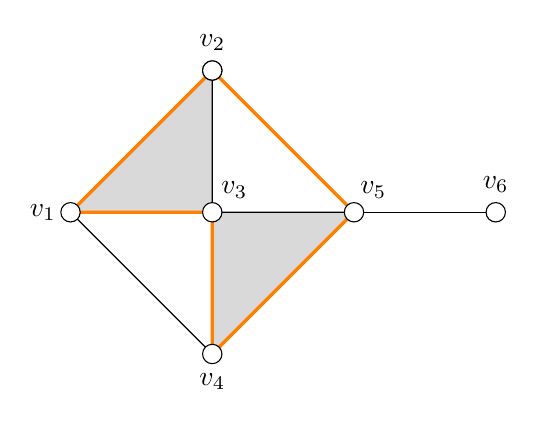
\begin{tikzpicture}[
            scale = .6,
            every node/.style={
              circle,
              draw=black,
              fill=white,
              inner sep=0pt,
              minimum size=7pt
            }
            ]

            \coordinate (v1) at (-3,0);
            \coordinate (v2) at (0,3);
            \coordinate (v3) at (0,0);
            \coordinate (v4) at (0,-3);
            \coordinate (v5) at (3,0);
            \coordinate (v6) at (6,0);

            \draw[fill=gray!30!white] (v1) -- (v2) -- (v3) -- (v1) -- cycle;
            \draw[fill=gray!30!white] (v3) -- (v4) -- (v5) -- (v3) -- cycle;

            \draw (v1) -- (v4);
            \draw (v2) -- (v5);
            \draw (v5) -- (v6);

            \draw[draw=orange, very thick] (v1) -- (v2) -- (v5) -- (v4)-- (v3) -- cycle;

            \node (wv1) at (v1) {};
            \node (wv2) at (v2) {};
            \node (vv2) at (v2) {};
            \node (vv3) at (v3) {};
            \node (vv4) at (v4) {};
            \node (vv5) at (v5) {};
            \node (vv6) at (v6) {};

            \node[draw=none, xshift=-1em] (wv1) at (v1) {$v_1$};
            \node[draw=none, yshift=1em] (wv2) at (v2) {$v_2$};
            \node[draw=none, xshift=.8em, yshift=.8em] (wv3) at (v3) {$v_3$};
            \node[draw=none, yshift=-1em] (wv4) at (v4) {$v_4$};
            \node[draw=none, xshift=.7em, yshift=.8em] (wv5) at (v5) {$v_5$};
            \node[draw=none, yshift=1em] (wv6) at (v6) {$v_6$};
          \end{tikzpicture}
        \end{subfigure}
        \begin{subfigure}{.49\linewidth}
          \centering
          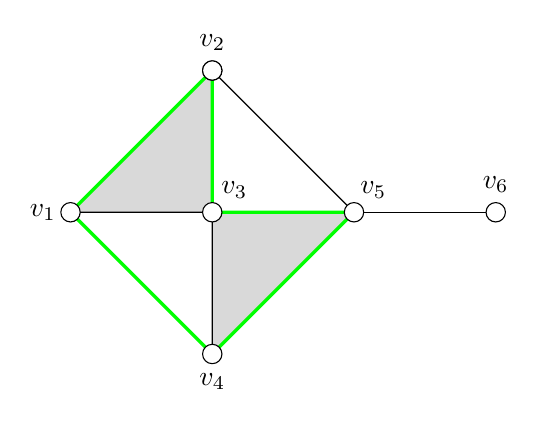
\begin{tikzpicture}[
            scale = .6,
            every node/.style={
              circle,
              draw=black,
              fill=white,
              inner sep=0pt,
              minimum size=7pt
            }
            ]

            \coordinate (v1) at (-3,0);
            \coordinate (v2) at (0,3);
            \coordinate (v3) at (0,0);
            \coordinate (v4) at (0,-3);
            \coordinate (v5) at (3,0);
            \coordinate (v6) at (6,0);

            \draw[fill=gray!30!white] (v1) -- (v2) -- (v3) -- (v1) -- cycle;
            \draw[fill=gray!30!white] (v3) -- (v4) -- (v5) -- (v3) -- cycle;

            \draw (v1) -- (v4);
            \draw (v2) -- (v5);
            \draw (v5) -- (v6);

            \draw[draw=green, very thick] (v1) -- (v2) -- (v3) -- (v5) -- (v4) -- cycle;

            \node (wv1) at (v1) {};
            \node (wv2) at (v2) {};
            \node (vv2) at (v2) {};
            \node (vv3) at (v3) {};
            \node (vv4) at (v4) {};
            \node (vv5) at (v5) {};
            \node (vv6) at (v6) {};

            \node[draw=none, xshift=-1em] (wv1) at (v1) {$v_1$};
            \node[draw=none, yshift=1em] (wv2) at (v2) {$v_2$};
            \node[draw=none, xshift=.8em, yshift=.8em] (wv3) at (v3) {$v_3$};
            \node[draw=none, yshift=-1em] (wv4) at (v4) {$v_4$};
            \node[draw=none, xshift=.7em, yshift=.8em] (wv5) at (v5) {$v_5$};
            \node[draw=none, yshift=1em] (wv6) at (v6) {$v_6$};
          \end{tikzpicture}
        \end{subfigure}
        \begin{subfigure}{.49\linewidth}
          \centering
          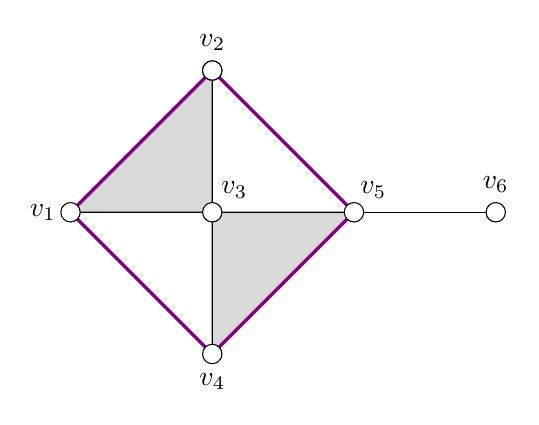
\begin{tikzpicture}[
            scale = .6,
            every node/.style={
              circle,
              draw=black,
              fill=white,
              inner sep=0pt,
              minimum size=7pt
            }
            ]

            \coordinate (v1) at (-3,0);
            \coordinate (v2) at (0,3);
            \coordinate (v3) at (0,0);
            \coordinate (v4) at (0,-3);
            \coordinate (v5) at (3,0);
            \coordinate (v6) at (6,0);

            \draw[fill=gray!30!white] (v1) -- (v2) -- (v3) -- (v1) -- cycle;
            \draw[fill=gray!30!white] (v3) -- (v4) -- (v5) -- (v3) -- cycle;

            \draw (v1) -- (v4);
            \draw (v2) -- (v5);
            \draw (v5) -- (v6);

            \draw[draw=violet, very thick] (v1) -- (v2) -- (v5) -- (v4) -- cycle;

            \node (wv1) at (v1) {};
            \node (wv2) at (v2) {};
            \node (vv2) at (v2) {};
            \node (vv3) at (v3) {};
            \node (vv4) at (v4) {};
            \node (vv5) at (v5) {};
            \node (vv6) at (v6) {};

            \node[draw=none, xshift=-1em] (wv1) at (v1) {$v_1$};
            \node[draw=none, yshift=1em] (wv2) at (v2) {$v_2$};
            \node[draw=none, xshift=.8em, yshift=.8em] (wv3) at (v3) {$v_3$};
            \node[draw=none, yshift=-1em] (wv4) at (v4) {$v_4$};
            \node[draw=none, xshift=.7em, yshift=.8em] (wv5) at (v5) {$v_5$};
            \node[draw=none, yshift=1em] (wv6) at (v6) {$v_6$};
          \end{tikzpicture}
        \end{subfigure}
        \begin{subfigure}{.49\linewidth}
          \centering
          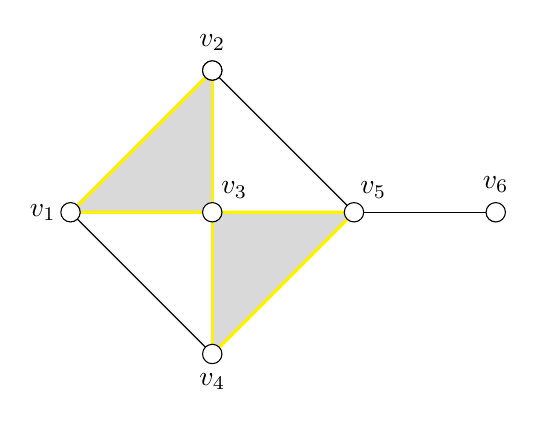
\begin{tikzpicture}[
            scale = .6,
            every node/.style={
              circle,
              draw=black,
              fill=white,
              inner sep=0pt,
              minimum size=7pt
            }
            ]

            \coordinate (v1) at (-3,0);
            \coordinate (v2) at (0,3);
            \coordinate (v3) at (0,0);
            \coordinate (v4) at (0,-3);
            \coordinate (v5) at (3,0);
            \coordinate (v6) at (6,0);

            \draw[fill=gray!30!white] (v1) -- (v2) -- (v3) -- (v1) -- cycle;
            \draw[fill=gray!30!white] (v3) -- (v4) -- (v5) -- (v3) -- cycle;

            \draw (v1) -- (v4);
            \draw (v2) -- (v5);
            \draw (v5) -- (v6);

            \draw[draw=yellow, very thick] (v1) -- (v2) -- (v3) -- cycle;
            \draw[draw=yellow, very thick] (v3) -- (v4) -- (v5) -- cycle;

            \node (wv1) at (v1) {};
            \node (wv2) at (v2) {};
            \node (vv2) at (v2) {};
            \node (vv3) at (v3) {};
            \node (vv4) at (v4) {};
            \node (vv5) at (v5) {};
            \node (vv6) at (v6) {};

            \node[draw=none, xshift=-1em] (wv1) at (v1) {$v_1$};
            \node[draw=none, yshift=1em] (wv2) at (v2) {$v_2$};
            \node[draw=none, xshift=.8em, yshift=.8em] (wv3) at (v3) {$v_3$};
            \node[draw=none, yshift=-1em] (wv4) at (v4) {$v_4$};
            \node[draw=none, xshift=.7em, yshift=.8em] (wv5) at (v5) {$v_5$};
            \node[draw=none, yshift=1em] (wv6) at (v6) {$v_6$};
          \end{tikzpicture}
        \end{subfigure}
        \caption{Some cycles in $K$}
      \end{figure}
    \item First, consider the following diagram:
      \begin{figure}[H]
        \centering
        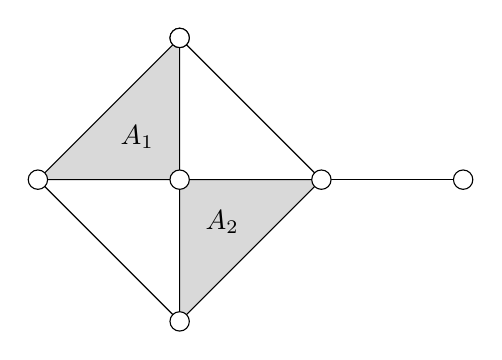
\begin{tikzpicture}[
          scale = .6,
          every node/.style={
            circle,
            draw=black,
            fill=white,
            inner sep=0pt,
            minimum size=7pt
          }
          ]

          \coordinate (v1) at (-3,0);
          \coordinate (v2) at (0,3);
          \coordinate (v3) at (0,0);
          \coordinate (v4) at (0,-3);
          \coordinate (v5) at (3,0);
          \coordinate (v6) at (6,0);

          \draw[fill=gray!30!white] (v1) -- (v2) -- (v3) -- (v1) -- cycle;

          \draw (v1) -- (v4);

          \draw[fill=gray!30!white] (v3) -- (v4) -- (v5) -- (v3) -- cycle;


          \draw (v2) -- (v5) ;
          \draw (v5) -- (v6) ;

          \node (wv1) at (v1) {};
          \node (wv2) at (v2) {};
          \node (vv2) at (v2) {};
          \node (vv3) at (v3) {};
          \node (vv4) at (v4) {};
          \node (vv5) at (v5) {};
          \node (vv6) at (v6) {};

          \node[draw=none,fill=none] (a1) at (-.9,.9) {$A_1$};
          \node[draw=none,fill=none] (a1) at (.9,-.9) {$A_2$};
        \end{tikzpicture}
        \caption{Two $n=2$ simplices}
      \end{figure}
      $\mb 0_1$ bounds $\mb 0_2$. Since $\partial(A_1) \cap \partial(A_2) =
      \varnothing$, then the other two cycles in $\msf B_1(K)$ are just
      $\partial(A_1)$ and $\partial(A_2)$, respectively.
    \item $\msf H_1(K) \cong \zmod{2} \times \zmod{2}$ (equivalence classes
      have representative elements $\mb 0, \partial(A_1), \partial(A_2),
      \partial(A_1) + \partial(A_2)$)
    \end{enumerate}
  \item For $k=2$, we have
    \begin{enumerate}
    \item $\msf C_2(K) \cong \zmod{2} \times \zmod{2}$
    \item $\msf Z_2(K) \cong \mb 0$
    \item $\msf B_2(K) \cong \mb 0$
    \item And hence $\msf H_2(K) \cong \mb 0$.
    \end{enumerate}
  \end{enumerate}
\end{solution}
\begin{problem}[16.7]
  If $K$ is a one-point space, $\msf H_n(K) \cong 0$ for $n \geq 0$, and $\msf
  H_0(K) \cong \zmod{2}$.
\end{problem}
\begin{solution}
  For $n > 0$, $\msf C_n(K)$ is the trivial group. Since $\msf Z_n(K) \leq \msf
  C_n(K)$, we thus have $\msf Z_n(K) \cong 0$, and so $\msf H_n(K) \cong 0$.

  For the $n = 0$, note that $\msf Z_0(K) = \msf C_0(K) \cong \zmod{2}$ (every
  point is definitionally a 0-cycle). Since $K$ contains no 1-simplices, $\msf
  B_0(K) = \mb 0$, hence $\msf H_0(K) \cong \zmod{2}$.
\end{solution}
\begin{definition}[Acyclic]
  Any space with the homology groups of a point is called \emph{acyclic}.
\end{definition}
\begin{definition}[Simplicially connected]
  Let $K$ be a simplicial complex. Then we call $K$ \emph{simplicially
    connected} iff for all pairs of 0-simplices $v_0, v_n \in K$, there exists a
  sequence of 0-simplices $\set{v_i}_{i\in [n]}$ such that for all $i \in [n]$
  (with $i \neq n$), $\set{v_iv_{i+1}}$ is a 1-simplex in $K$. Note, this
  corresponds exactly to $K$ being connected as a graph, where the 0-simplices
  represent vertices, and the 1-simplices represent edges.
\end{definition}
\begin{problem}[16.8]
  If $K$ is simplicially connected, then $\msf H_0(K) \cong \zmod{2}$. If $K$
  has $r$ simplicially connected components, then
  \[
    \msf H_0(K)\cong \prod_{i=1}^r \zmod{2}
  \]
\end{problem}
\begin{solution}
  \begin{enumerate}
  \item Suppose $K$ is simplicially connected. We want to show $\msf H_0(K)
    \cong \zmod{2}$. First, observe that $\msf Z_0(K) \cong \msf C_0(K)$
    (every 0 simplex has trivial boundary). By properties of module
    homomorphisms, for all $\sigma \in \msf B_0(K)$, $\sigma$ is a basis
    element of $\msf B_0(K)$ iff $\exists \tau \in \msf C_1(K)$ such that
    $\tau$ is a basis element of $\msf C_1(K)$, and $\partial_1(\tau) =
    \sigma$. Thus, $\msf B_0(K)$ is spanned by $\set{\set{\set{v_i} +
        \set{v_j}} \MID \set{v_iv_j} \in K}$. It follows that $\msf B_0(K)$
    contains exactly those elements of $\msf C_0(K)$ with an even number of
    vertices.\footnote{Since $\msf B_0(K)$ is generated by pairs.}

    It follows that $\msf H_0(K) = \msf Z_0(K)/\msf B_0(K) \cong \zmod{2}$
    (any $0$-chain has either an even or odd number of vertices).
  \item This follows by applying the above argument to each of the connected
    components.
  \end{enumerate}
\end{solution}
\begin{problem}[16.9]
  Let $K$ be a triangulation of a $3$-dimensional ball that consists of a
  3-simplex together with its faces. Compute $\msf H_n(K)$ for each $n$.
\end{problem}
\begin{solution}
  \begin{figure}[H]
    \centering
    \begin{subfigure}{\linewidth}
      \centering
      \tdplotsetmaincoords{70}{80}
      \begin{tikzpicture}[tdplot_main_coords,scale=2]
        \path
        coordinate (A) at (0,0,0)
        coordinate (B) at (2,0,0)
        coordinate (C) at (1,1.732,0)
        coordinate (D) at (1,.577,1.733);

        \draw [dashed] (A)--(C);
        \fill [opacity=.5, red!30!white] (A) -- (B) -- (C) -- cycle;
        \fill [opacity=.5, blue!30!white] (D) -- (B) -- (A) -- cycle;
        \fill [opacity=.5, green!30!white] (D) -- (A) -- (C) -- cycle;
        \draw[thick] (A) -- (B) (A) -- (D);
        \draw[thick, fill opacity=.5, fill=orange!30!white] (D) -- (B) -- (C) -- cycle;

        \node (V) at (1,.577,.433) {\LARGE $V_1$};

        \foreach \v/\position in {A/left,B/below,C/right,D/above} {
          \draw[fill=black] (\v) circle (0.5pt) node [\position=0.2mm] {$\v$};
        }
      \end{tikzpicture}
    \end{subfigure}\\\vspace{1cm}
    \begin{subfigure}{.24\linewidth}
      \centering
      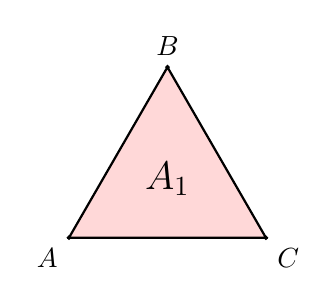
\begin{tikzpicture}[scale=1.25]
        \path
        coordinate (A) at (0,0)
        coordinate (C) at (2,0)
        coordinate (B) at (1,1.732);

        \draw[thick, fill opacity=.5, fill=red!30!white] (A) -- (B) -- (C) -- cycle;

        \node (A1) at (1,.6) {\Large $A_1$};

        \foreach \v/\position in {A/below left, C/below right, B/above} {
          \draw[fill=black] (\v) circle (0.5pt) node [\position=0.2mm] {$\v$};
        }
      \end{tikzpicture}
    \end{subfigure}
    \begin{subfigure}{.24\linewidth}
      \centering
      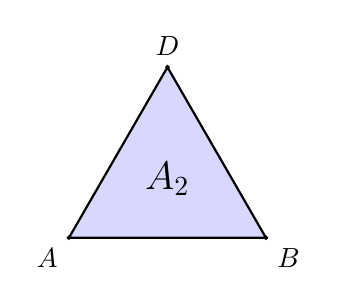
\begin{tikzpicture}[scale=1.25]
        \path
        coordinate (A) at (0,0)
        coordinate (B) at (2,0)
        coordinate (D) at (1,1.732);

        \draw[thick, fill opacity=.5, fill=blue!30!white] (D) -- (B) -- (A) -- cycle;

        \node (A2) at (1,.6) {\Large $A_2$};

        \foreach \v/\position in {A/below left, B/below right, D/above} {
          \draw[fill=black] (\v) circle (0.5pt) node [\position=0.2mm] {$\v$};
        }
      \end{tikzpicture}
    \end{subfigure}
    \begin{subfigure}{.24\linewidth}
      \centering
      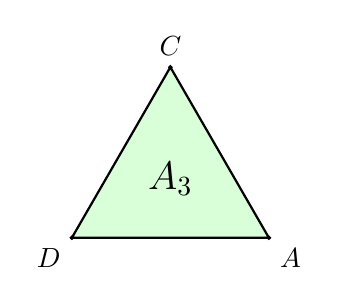
\begin{tikzpicture}[scale=1.25]
        \path
        coordinate (D) at (0,0)
        coordinate (A) at (2,0)
        coordinate (C) at (1,1.732);

        \draw[thick, fill opacity=.5, fill=green!30!white] (D) -- (A) -- (C) -- cycle;

        \node (A3) at (1,.6) {\Large $A_3$};

        \foreach \v/\position in {D/below left, A/below right, C/above} {
          \draw[fill=black] (\v) circle (0.5pt) node [\position=0.2mm] {$\v$};
        }
      \end{tikzpicture}
    \end{subfigure}
    \begin{subfigure}{.24\linewidth}
      \centering
      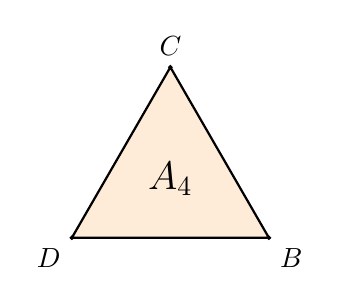
\begin{tikzpicture}[scale=1.25]
        \path
        coordinate (D) at (0,0)
        coordinate (B) at (2,0)
        coordinate (C) at (1,1.732);

        \draw[thick, fill opacity=.5, fill=orange!30!white] (D) -- (B) -- (C) -- cycle;

        \node (A4) at (1,.6) {\Large $A_4$};

        \foreach \v/\position in {D/below left, B/below right, C/above} {
          \draw[fill=black] (\v) circle (0.5pt) node [\position=0.2mm] {$\v$};
        }
      \end{tikzpicture}
    \end{subfigure}\\\vspace{1cm}
    \tikzset{
      brace/.style={
        thick,
        decoration={brace, mirror, raise=1pt, amplitude=6pt},
        decorate
      },
      blabel/.style={
        right, pos=.5, xshift=7pt, yshift=-2pt
      }
    }
    \begin{subfigure}{.161\linewidth}
      \centering
      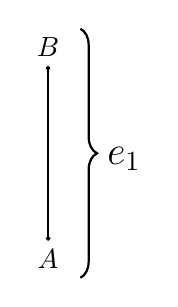
\begin{tikzpicture}[scale=1.25]
        \def\firstcoord{A}
        \def\secondcoord{B}
        \path coordinate (\firstcoord) at (0,0) coordinate (\secondcoord) at (0,1.73);
        \draw[thick] (\firstcoord) -- (\secondcoord);

        \draw[brace] (.3,-.4) -- node[blabel] {\Large $e_1$} (.3,2.13);

        \foreach \v/\position in {\firstcoord/below, \secondcoord/above} {
          \draw[fill=black] (\v) circle (0.5pt) node [\position=0.2mm] {$\v$};
        }
      \end{tikzpicture}
    \end{subfigure}
    \begin{subfigure}{.161\linewidth}
      \centering
      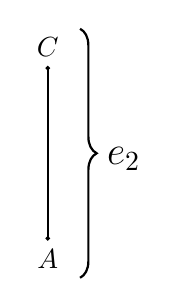
\begin{tikzpicture}[scale=1.25]
        \def\firstcoord{A}
        \def\secondcoord{C}
        \path coordinate (\firstcoord) at (0,0) coordinate (\secondcoord) at (0,1.73);
        \draw[thick] (\firstcoord) -- (\secondcoord);

        \draw[brace] (.3,-.4) -- node[blabel] {\Large $e_2$} (.3,2.13);

        \foreach \v/\position in {\firstcoord/below, \secondcoord/above} {
          \draw[fill=black] (\v) circle (0.5pt) node [\position=0.2mm] {$\v$};
        }
      \end{tikzpicture}
    \end{subfigure}
    \begin{subfigure}{.161\linewidth}
      \centering
      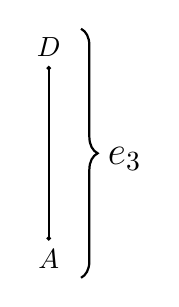
\begin{tikzpicture}[scale=1.25]
        \def\firstcoord{A}
        \def\secondcoord{D}
        \path coordinate (\firstcoord) at (0,0) coordinate (\secondcoord) at (0,1.73);
        \draw[thick] (\firstcoord) -- (\secondcoord);

        \draw[brace] (.3,-.4) -- node[blabel] {\Large $e_3$} (.3,2.13);

        \foreach \v/\position in {\firstcoord/below, \secondcoord/above} {
          \draw[fill=black] (\v) circle (0.5pt) node [\position=0.2mm] {$\v$};
        }
      \end{tikzpicture}
    \end{subfigure}
    \begin{subfigure}{.161\linewidth}
      \centering
      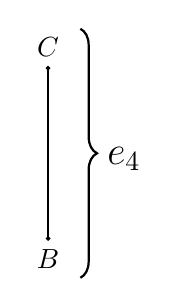
\begin{tikzpicture}[scale=1.25]
        \def\firstcoord{B}
        \def\secondcoord{C}
        \path coordinate (\firstcoord) at (0,0) coordinate (\secondcoord) at (0,1.73);
        \draw[thick] (\firstcoord) -- (\secondcoord);

        \draw[brace] (.3,-.4) -- node[blabel] {\Large $e_4$} (.3,2.13);

        \foreach \v/\position in {\firstcoord/below, \secondcoord/above} {
          \draw[fill=black] (\v) circle (0.5pt) node [\position=0.2mm] {$\v$};
        }
      \end{tikzpicture}
    \end{subfigure}
    \begin{subfigure}{.161\linewidth}
      \centering
      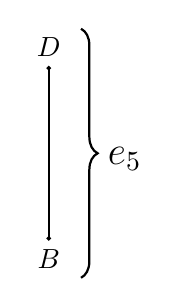
\begin{tikzpicture}[scale=1.25]
        \def\firstcoord{B}
        \def\secondcoord{D}
        \path coordinate (\firstcoord) at (0,0) coordinate (\secondcoord) at (0,1.73);
        \draw[thick] (\firstcoord) -- (\secondcoord);

        \draw[brace] (.3,-.4) -- node[blabel] {\Large $e_5$} (.3,2.13);

        \foreach \v/\position in {\firstcoord/below, \secondcoord/above} {
          \draw[fill=black] (\v) circle (0.5pt) node [\position=0.2mm] {$\v$};
        }
      \end{tikzpicture}
    \end{subfigure}
    \begin{subfigure}{.161\linewidth}
      \centering
      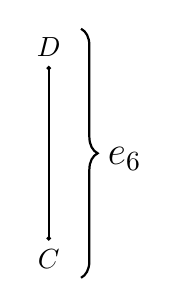
\begin{tikzpicture}[scale=1.25]
        \def\firstcoord{C}
        \def\secondcoord{D}
        \path coordinate (\firstcoord) at (0,0) coordinate (\secondcoord) at (0,1.73);
        \draw[thick] (\firstcoord) -- (\secondcoord);

        \draw[brace] (.3,-.4) -- node[blabel] {\Large $e_6$} (.3,2.13);

        \foreach \v/\position in {\firstcoord/below, \secondcoord/above} {
          \draw[fill=black] (\v) circle (0.5pt) node [\position=0.2mm] {$\v$};
        }
      \end{tikzpicture}
    \end{subfigure}\\\vspace{1.5cm}
    \begin{subfigure}{\linewidth}
      \centering
      \begin{tikzpicture}[scale=1.25]
        \path
        coordinate (A) at (-4,0)
        coordinate (B) at (-1.33,0)
        coordinate (C) at (1.33,0)
        coordinate (D) at (4,0);

        \foreach \v in {A,B,C,D} {
          \draw[fill=black] (\v) circle (2pt) node [below, yshift=-5pt] {$\v$};
        }
      \end{tikzpicture}
    \end{subfigure}\\\vspace{0cm}
    \caption{3-simplex and its basis faces. Note the 1, 4, 6, 4 relationship.
      Gotta love Pascal's 2-simplex!}
    \label{fig:circumscribed}
  \end{figure}
  \begin{enumerate}[label=(\arabic*)]\setcounter{enumi}{-1}
  \item $K$ is connected, so $\msf H_0(K) \cong \mb \zmod{2}$.
  \item Elements of $\msf Z_1(K)$ are all just closed loops (linear combinations
    of the $\bdy[2]{A_i}$). But elements of $\msf B_1(K)$ are also just linear
    combinations of the $\bdy[2]{A_i}$. Hence $\msf H_1(K) \cong \mb 0$.
  \item $\msf Z_2(K) = \set{\mb 0, A_1 + A_2 + A_3 + A_4} = B_2(K) \cong
    \zmod{2}$, so $\msf H_2(K) \cong \mb 0$.
  \item $\msf H_3(K) \cong \mb 0$.
  \end{enumerate}
  It follows that the 3-simplex with all its faces is acyclic, which makes
  sense, since the underlying space is homeomorphic to the 3-ball, and the
  3-ball is homeomorphic to a point.
\end{solution}
\begin{problem}[16.10]
  Let $K$ be a triangulation of a 2-sphere that consists of the proper faces of
  a 3-simplex. Compute $\msf H_n(K)$ for each $n$.
\end{problem}
\begin{solution}
  Proceed as before for $k=0,1$. For $k=2$, note $\msf B_2(K) \cong \mb 0$.
  Hence, $\msf H_2(K) \cong \zmod{2}$.
\end{solution}
\begin{definition}[Seeing a simplex]
  Let $K$ be a simplicial complex with $\abs{K} \subset \RR^n$. A point $x
  \not\in K$ can \emph{see} $K$ if any ray from $x$ intersects $\abs{K}$ at most
  once (as seen in the following diagram).
\end{definition}
\begin{figure}[H]
  \centering
  \begin{subfigure}{.49\linewidth}
    \centering
    \tdplotsetmaincoords{70}{80}
    \begin{tikzpicture}[tdplot_main_coords, scale=2]
      \path
      coordinate (B) at (2,0,0)
      coordinate (C) at (1,1.732,0)
      coordinate (x) at (.6,.577,1.533)
      coordinate (y) at (1.8,1.077,1.733);

      \draw (B)--(C);

      \path
      coordinate (P1) at ($.5*(B) + .5*(C)$)
      coordinate (P2) at ($.23*(B) + .77*(C)$)
      coordinate (P3) at ($.7*(B) + .3*(C)$)
      coordinate (P4) at ($.4*(B) + .6*(C)$);

      \foreach \v in {P1,P2,P3,P4}{
        % Take the difference and go slightly past it
        \draw[-latex,dashed,color=red!30!white] (x) -- ($1.3*(\v) - .3*(x)$);
        \draw[-latex,dashed,color=blue!30!white] (y) -- ($1.3*(\v) - .3*(y)$);
        \draw[fill=black] (\v) circle (0.5pt);
      }

      \foreach \v in {B,C}{
        % Take the difference and go slightly past it
        \draw[-latex,dashed,color=red!30!white] (x) -- ($1.2*(\v) - .2*(x)$);
        \draw[-latex,dashed,color=blue!30!white] (y) -- ($1.2*(\v) - .2*(y)$);
        \draw[fill=black] (\v) circle (0.5pt);
      }

      \foreach \v/\position in {B/left,C/right,x/above,y/above right} {
        \draw[fill=black] (\v) circle (0.5pt) node [\position=0.2mm] {$\v$};
      }
    \end{tikzpicture}
    \caption{$x$ and $y$ both see a $1$-simplex $\sigma_1$}
    \label{fig:see-sigma-1}
  \end{subfigure}
  \begin{subfigure}{.49\linewidth}
    \centering
    \tdplotsetmaincoords{70}{80}
    \begin{tikzpicture}[tdplot_main_coords, scale=2]
      \path
      coordinate (A) at (0,0,0)
      coordinate (B) at (2,0,0)
      coordinate (C) at (1,1.732,0)
      coordinate (x) at (1,.577,1.733);

      \fill[red!30!white,draw=black] (A)--(B)--(C)--cycle;

      \path
      coordinate (P1) at ($.2*(A) + .5*(B) + .4*(C)$)
      coordinate (P2) at ($.3*(A) + .5*(B) + .2*(C)$)
      coordinate (P3) at ($.2*(A) + .2*(B) + .6*(C)$)
      coordinate (P4) at ($.7*(A) + .2*(B) + .1*(C)$);

      \foreach \v in {P1,P2,P3,P4}{
        % Take the difference and go slightly past it
        \draw[-latex,dashed] (x) -- ($1.3*(\v) - .3*(x)$);
        \draw[fill=black] (\v) circle (0.5pt);
      }

      \foreach \v in {A,B,C}{
        % Take the difference and go slightly past it
        \draw[-latex,dashed] (x) -- ($1.2*(\v) - .2*(x)$);
        \draw[fill=black] (\v) circle (0.5pt);
      }

      \foreach \v/\position in {A/left,B/left,C/right,x/above} {
        \draw[fill=black] (\v) circle (0.5pt) node [\position=0.2mm] {$\v$};
      }
    \end{tikzpicture}
    \caption{$x$ sees a $2$-simplex $\sigma_2$}
    \label{fig:see-sigma-2}
  \end{subfigure}
  \caption{Simplices being seen}
  \label{fig:seeing}
\end{figure}
\begin{remark}
  Note, that when there are multiple $k$-simplices in $K$, the picture might not
  be quite as simple.
\end{remark}
\begin{remark}
  As far as I can tell, a point $x$ sees $K$ iff $x$ is in orthogonal complement
  of the $k$-hyperplane containing $K$. Not sure if this is actually correct
  though?
\end{remark}
\begin{definition}[Cone of $x$ over $\sigma$]
  Let $K$ be a finite complex and $x$ a point that sees $K$. If $\sigma =
  \simp{k}$ is a simplex of $K$, define the \emph{cone} of $x$ over $\sigma$ to
  be the simplex
  \[
    \Cone_x(\sigma) = \set{xv_0\cdots v_k}.
  \]
\end{definition}
\begin{figure}[H]
  \centering
  \begin{subfigure}{.49\linewidth}
    \centering
    \tdplotsetmaincoords{70}{80}
    \begin{tikzpicture}[tdplot_main_coords, scale=2]
      \path
      coordinate (B) at (2,0,0)
      coordinate (C) at (1,1.732,0)
      coordinate (x) at (.6,.577,1.533)
      coordinate (y) at (1.8,1.077,1.733);

      \draw (B)--(C);

      \fill [opacity=.5, red!30!white] (x) -- (B) -- (C) -- cycle;
      \fill [opacity=.5, blue!30!white] (y) -- (B) -- (C) -- cycle;

      \draw[dotted] (x) -- (B) (x) -- (C);
      \draw[dotted] (y) -- (B) (y) -- (C);

      \foreach \v/\position in {B/left,C/right,x/above,y/above right} {
        \draw[fill=black] (\v) circle (0.5pt) node [\position=0.2mm] {$\v$};
      }
    \end{tikzpicture}
    \caption{$\Cone_x(\sigma_1)$, $\Cone_y(\sigma_1)$}
    \label{fig:cone-sigma-1}
  \end{subfigure}
  \begin{subfigure}{.49\linewidth}
    \centering
    \tdplotsetmaincoords{70}{80}
    \begin{tikzpicture}[tdplot_main_coords, scale=2]
      \path
      coordinate (A) at (0,0,0)
      coordinate (B) at (2,0,0)
      coordinate (C) at (1,1.732,0)
      coordinate (x) at (1,.577,1.733);

      \fill[red!30!white,draw=black] (A)--(B)--(C)--cycle;

      % Draw this first so it gets covered by the fill slightly
      \draw (A) -- (C);

      \fill [opacity=.8, red!50!white] (A) -- (B) -- (C) -- cycle;
      \fill [opacity=.4, blue!30!white] (x) -- (B) -- (A) -- cycle;
      \fill [opacity=.4, blue!30!white] (x) -- (A) -- (C) -- cycle;
      \fill [opacity=.4, blue!30!white] (x) -- (B) -- (C) -- cycle;
      \draw[dotted] (A) -- (x) (B) -- (x) (C) -- (x);

      % Draw this first so it gets covered by the fill slightly
      \draw (A) -- (B) -- (C);

      \foreach \v/\position in {A/left,B/left,C/right,x/above} {
        \draw[fill=black] (\v) circle (0.5pt) node [\position=0.2mm] {$\v$};
      }
    \end{tikzpicture}
    \caption{$\Cone_x(\sigma_2)$}
    \label{fig:cone-sigma-2}
  \end{subfigure}
  \caption{Some cones}
  \label{fig:cones}
\end{figure}
\begin{definition}[Cone over $K$]
  Define $x*K$, the \emph{cone over} $K$ to be the simplicial complex comprising
  all simplices $\Cone_x(\sigma)$ for $\sigma \in K$, and all faces of such
  simplices.
\end{definition}
\begin{remark}
  Essentially, this just includes the base point and edges in
  \cref{fig:cone-sigma-1} and the base point and edges \emph{and} faces in
  \cref{fig:cone-sigma-2}.
\end{remark}
\begin{figure}[H]
  \centering
  \tdplotsetmaincoords{70}{80}
  \begin{tikzpicture}[tdplot_main_coords, scale=2]
    \path
    coordinate (A) at (0,0,0)
    coordinate (B) at (2,0,0)
    coordinate (C) at (1,1.732,0)
    coordinate (D) at (1,.577,1.733);

    \fill[red!30!white,draw=black] (A)--(B)--(C)--cycle;

    % Draw this first so it gets covered by the fill slightly
    \draw (A) -- (C);

    \fill [opacity=.5, red!30!white] (A) -- (B) -- (C) -- cycle;
    \fill [opacity=.5, blue!30!white] (D) -- (B) -- (A) -- cycle;
    \fill [opacity=.5, green!30!white] (D) -- (A) -- (C) -- cycle;
    \fill [opacity=.5, orange!30!white] (D) -- (B) -- (C) -- cycle;
    \draw[dashed] (A) -- (D) (B) -- (D) (C) -- (D);

    % Draw this first so it gets covered by the fill slightly
    \draw (A) -- (B) -- (C);

    \foreach \v/\position in {A/left,B/left,C/right,D/above} {
      \draw[fill=black] (\v) circle (0.5pt) node [\position=0.2mm] {$\v$};
    }
  \end{tikzpicture}
  \caption{$x * \sigma_2$. Note, each of the faces is colored to indicate
    inclusion in the complex.}
  \label{fig:cone-over-sigma-2}
\end{figure}
\begin{definition}[Simplicial cone operator]
  Define the \emph{simplicial cone operator} $\Cone_x : \msf C_n(K) \to \msf
  C_{n+1}(x*K)$ by extending the definition of $\Cone_x(\sigma)$ linearly to
  chains.
\end{definition}
\begin{problem}[16.11]
  For $x$ seeing $K$, and $\sigma$ a simplex of $K$,
  \[
    \partial\, \Cone_x(\sigma) + \Cone_x(\partial \sigma) = \sigma.
  \]
\end{problem}
\begin{solution}
  Let $\sigma = \simp{k}$. Then
  \begin{align*}
    \partial\, \Cone_x(\sigma) + \Cone_x(\partial \sigma)
    &= \pn{\set{\widehat{x}v_0\cdots v_k} + \sum_{i\in [k]} \simpdel{i}{k}} + \Cone_x \pn{\sum_{i\in [k]} \simpdel{i}{k}} \\
    &= \sigma + \sum_{i\in [k]} \simpdel{i}{k} + \simpdel{i}{k} \\
    &= \sigma + \sum_{i \in [k]} \mb 0 \\
    &= \sigma
  \end{align*}
  as desired.
\end{solution}
\begin{problem}[16.12]
  For any complex $K$ and $x$ seeing $K$, the complex $x*K$ is acyclic.
\end{problem}
\begin{solution}

\end{solution}
\begin{problem}[16.13]

\end{problem}
\begin{solution}

\end{solution}
\section{Induced Homomorphisms and Invariance}
Fix two simplicial complexes $K$ and $L$.
\begin{problem}[16.14]
  Let $f : K \to L$ be a simplicial map. Carefully write out the definition of
  the natural induced map from $n$-chains of $K$ to $n$-chains of $L$:
  \[
    f_{\# n} : \msf C_n(K) \to \msf C_n(L)
  \]
  and show that it is a homomorphism.
\end{problem}
\begin{solution}
  We define $f_\#$ by its action on basis elements, then apply linear extension.
  Let $\sigma = \simp{n} \in \msf C_n(K)$ be a basis element. Then define
  \[
    f_{\# n}(\sigma) =
    \begin{cases}
      \mb 0 & \text{if $f(\sigma)$ is not a $n$-simplex, and }\\
      f(\sigma) & \text{otherwise}
    \end{cases}
  \]
  We now apply linear extension. That is, for all $\tau = \sum_{i \in I}
  \simp[v^{(i)}]{n} \in \msf C_n(K)$, define
  \begin{align*}
    f_{\# n}(\tau)
    &= f_{\# n} \pn{\sum_{i\in I} \sigma_i} \\
    &= \sum_{i\in I} f_{\# n}(\sigma_i)
    % \\
    % &= \sum_{i \in I} f_{\# n}\pn{\simp[v^{(i)}]{n}} \\
    % &= \sum_{i \in I} \set{f\pn{v_0^{(i)}}\cdots f\pn{v_n^{(i)}}}
  \end{align*}
  we want to show this is a homomorphism.
  \begin{enumerate}[label=(\arabic*)]
  \item Let $\sigma_1, \sigma_2 \in \msf C_n(K)$ be arbitrary. Then
    \begin{align*}
      f_{\# n}\pn{\sigma_1 + \sigma_2}
      &= f_{\# n} \pn{\sum_{k\in I \cup J} \simp[v^{(k)}]{n}} \\
      &= f_{\# n} \pn{\sum_{i\in I} \simp[v^{(i)}]{n} + \sum_{j \in J} \simp[v^{(j)}]{n}} \\
      &= f_{\# n} \pn{\sum_{i\in I} \simp[v^{(i)}]{n}} + f_{\# n}\pn{\sum_{j \in J} \simp[v^{(j)}]{n}} \\
      &= f_{\# n}(\sigma_1) + f_{\# n}(\sigma_2)
    \end{align*}
  \item We want to show $f_{\# n}(\mb 0) = \mb 0$. Note, for any $\sigma \in
    \msf C_n(K)$, $\mb 0 = \sigma + \sigma$. By linearity, $f_{\# n}(\mb 0) =
    f_{\# n}(\sigma + \sigma) = f_{\# n}(\sigma) + f_{\# n}(\sigma) = \mb 0$
    as well, as desired.
  \end{enumerate}
  thus $f_{\# n}$ is a homomorphism.
\end{solution}
The map $f_{\# n}$ is called the \emph{induced chain map.} The next exercise
contains an important technicality about the induced chain map in the case where
the image of an $n$-simplex is an $(n-1)$-simplex.
\begin{problem}[16.15]
  If the simplicial map $f : K \to L$ maps an $n$-simplex $\sigma$ to an
  $(n-1)$-simplex $\tau$, what is $f_{\# n}(\sigma)$?
\end{problem}
\begin{solution}
  By the definition given above, $f_{\# n}(\sigma) = \mb 0$.
\end{solution}
\begin{problem}[16.16]
  Let $f : K \to L$ be a simplicial map, and let $f_\#$ be the induced map $f_\#
  : \msf C_n(K) \to \msf C_n(L)$. Then for any chain $c \in \msf C_n(K)$,
  \[
    \partial (f_\# (c)) = f_{\#}(\partial(c))
  \]
  In other ``words,'' we have the following commutative diagram
  \begin{figure}[H]
    \centering
    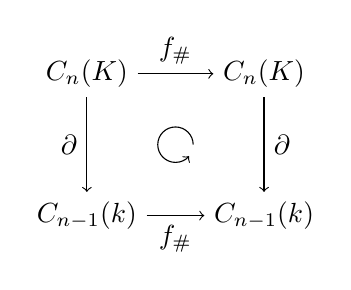
\begin{tikzpicture}[scale=.9]
      \node (00) at (0,0) {$\msf C_n(K)$};
      \node (10) at (2.5,0) {$\msf C_{n}(K)$};
      \node (01) at (0,-2) {$\msf C_{n-1}(k)$};
      \node (11) at (2.5,-2) {$\msf C_{n-1}(k)$};
      \draw[->] (00) -- node[above] {$f_\#$} (10);
      \draw[->] (01) -- node[below] {$f_\#$} (11);
      \draw[->] (00) -- node[left] {$\partial$} (01);
      \draw[->] (10) -- node[right] {$\partial$} (11);
      \draw[->] (1.5, -1) arc (0:320:.25cm);
    \end{tikzpicture}
    \caption{Commutative diagram}
  \end{figure}
\end{problem}
\begin{solution}
  Let $c \in \msf C_n(K)$. Express $c$ as a sum of basis elements
  $\set{\sigma}_{i \in I}$. Let $\set{\sigma_i}_{i \in I'}$ be those $\sigma_i$
  for which $f_{\#}(\sigma_i) \neq \mb 0$. Then
  \begin{align*}
    \partial_{n} (f_{\# n}(c))
    &= \partial_n \pn{\sum_{i\in I'} f_{\# n}(\sigma_i)} \\
    &= \partial_n \pn{\sum_{i \in I'} f(\sigma_i)} \\
    &= \partial_n \pn{\sum_{i\in I'} \set{f\pn{v_0^{(i)}}\cdots f\pn{v_n^{(i)}}}} \\
    &= \sum_{i\in I'} \sum_{j=1}^n \set{f\pn{v_0^{(i)}}\cdots \widehat{f\pn{v_j^{(i)}}}\cdots f\pn{v_n^{(i)}}} \\
    &= \sum_{i \in I'} \sum_{j=1}^n f_{\# n-1} \pn{\simpdel[v^{(i)}]{j}{n}} \\
    &= \sum_{i \in I'} f_{\# n-1}\pn{\partial \pn{\sigma_i}} \\
    &= f_{\# n-1} \pn{ \partial_n \pn{ \sum_{i \in I'} \sigma_i }} \\
    &= f_{\# n-1} \pn{ \partial_n \pn c} \\
  \end{align*}
  as desired.
\end{solution}
\begin{definition}[Induced Homomorphism]
  Let $f : K \to L$ be a simplicial map. The \emph{induced homomorphism} $f_* :
  \msf H_n(K) \to \msf H_n(L)$ is defined by $f_*([z]) = [f_\#(z)]$ (where the
  square brackets indicate an equivalence class).
\end{definition}
\begin{problem}[16.17]
  Let $f : K \to L$ be a simplicial map. Then the induced homomorphism $f_* :
  \msf H_n(K) \to \msf H_n(L)$ is a well-defined homomorphism.
\end{problem}
\begin{solution}
  That $f_*$ is a homomorphism follows directly from the definition.
  \begin{enumerate}[label=(\arabic*)]
  \item That $f_*([\mb 0]) = [\mb 0]$ follows by the definition of $f_{\#}$.
  \item Similarly for $f_*(\sigma + \tau) = f_*(\sigma) + f_*(\tau)$.
  \end{enumerate}
  We now show that $f_*$ is well-defined. Let $[\sigma] \in \msf H_n(K)$ and
  $[\tau] \in \msf H_n(K)$ with $[\sigma] = [\tau]$. Then $\exists \rho \in \msf
  B_n(K) \st \sigma = \tau + \rho$. Observe that
  \begin{align*}
    f_*([\sigma])
    &= [f_{\#}(\sigma)] \\
    &= [f_{\#}(\tau + \rho)] \\
    &= [f_{\#}(\tau) + f_{\#}(\rho)] \\
    &= [f_{\#}(\tau)] + [f_{\#}(\rho)] \\
    &= [f_{\#}(\tau)] + [\mb 0] \\
    &= [f_{\#}(\tau)],
  \end{align*}
  as desired.
\end{solution}
\begin{problem}[16.18]
  Let $K$ be a complex comprising the proper faces of a hexagon: six edges and
  six vertices $v_0, \ldots, v_5$. Let $L$ be the complex comprising the proper
  faces of a triangle: three edges and three vertices $w_0, w_1, w_2$. Let $f$
  be a simplicial map that sends $v_i$ to $w_{i \bmod 3}$. Compute the homology
  groups of $K$ and $L$ and describe the simplicial map $f$ and the induced
  homomorphism $f_*$.
\end{problem}
\begin{solution}
  \begin{enumerate}[label=(\arabic*)]
  \item We compute the homology groups of $K$. Observe, $\msf H_2(K) \cong
    \set{\mb 0}$ (since $\msf Z_n(K)$ is trivial). $\msf H_1(K) \cong
    \zmod{2}$ (since $\msf Z_1(K) \cong \zmod{2}$, as we either have the whole
    hexagon or we don't, and $\msf B_1(K) \cong \set{\mb 0}$). Finally, by
    theorem 16.8, we have $\msf H_0(K) \cong \zmod{2}$.
  \item The homology groups of $L$ are the same.
  \item The map $f$ folds the circle $\abs{K}$ onto itself
  \item $f_*$ is an isomorphism.
  \end{enumerate}
\end{solution}
\begin{definition}[$\lambda$-map]
  Let $K$ be a simplicial complex. Let $\lambda : \sd K \to K$ be defined as
  follows: for any vertex $v \in \sd K$, there exists $\sigma \in K$ such that
  $v$ is the barycenter of $\sigma$. Then let
  \[
    \lambda(v) = v_\sigma
  \]
  where $v_\sigma$ is a vertex in $\sigma$.
\end{definition}
\begin{definition}[$\lambda_*$]
  Let $\lambda_* : \msf H_n(\sd K) \to \msf H_n(K)$ be defined by linear
  extension of $\lambda$ to simplices. Since $\lambda$ is a well-defined
  simplicial map, $\lambda_*$ is a well-defined homomorphism (theorem 16.17).
\end{definition}
\begin{problem}[16.19]
  Suggest a homomorphism from $\msf C_n(K) \to \msf C_n(\sd K)$ that commutes
  with $\partial$. Could its induced homomorphism on homology be an inverse for
  $\lambda_*$?
\end{problem}
\begin{solution}
  Consdier $f : \msf C_n(K) \to \msf C_n(\sd K)$ defined by
  \[
    f(\sigma) = \text{sum of maximal $n$-simplices in $\sd \sigma$}
  \]
\end{solution}
We give this a name.
\begin{definition}[Subdivision operator]
  Define the \emph{subdivision operator} $\SD : \msf C_n(K) \to \msf C_n(\sd K)$
  by first defining $\SD$ on a simplex:
  \[
    \SD(\simp{n}) = \sum_{\mathclap{\pi \in \mc S_{n+1}}} \simp[b^{\pi}]{n}
  \]
  where $\mc S_{n+1}$ is the symmetric group, and $b_k^\pi$ is the barycenter of
  the face $\set{v_{\pi(0)}\cdots v_{\pi(k)}}$.
\end{definition}
\begin{note}
  I'm pretty sure this gets us all the maximal simplices, as we want. To verify
  it, I think we proceed as follows: let $\sigma \in \sd K$ be an arbitrary
  $n$-simplex. Then one of the vertices in $\sigma$ is a vertex in $K$ (def.\ of
  maximal simplex). Take $\pi$ such that $v_{\pi(0)}$ is this maximal vertex.
  Also restrict $\pi$ such that $v_{\pi(1)}$ is the vertex such that the
  barycenter of $\set{v_{\pi(0)}v_{\pi(1)}}$ is in $\sigma$ (again, since
  $\sigma$ is maximal, I think this works). Continue this.

  I think also that one can show this necessitates the resulting simplices be
  disjoint?
\end{note}
\begin{problem}[16.20]
  The subdivision operator commutes with the boundary operator, that is, if $c $
  is a chain in $K$, then $\SD(\partial c) = \partial \SD(c)$.
\end{problem}
\begin{solution}
  We show the result for a simplex. For intuition, observe the following
  diagram in the case $c$ is a $2$-simplex:
  \begin{figure}[H]
    \centering
    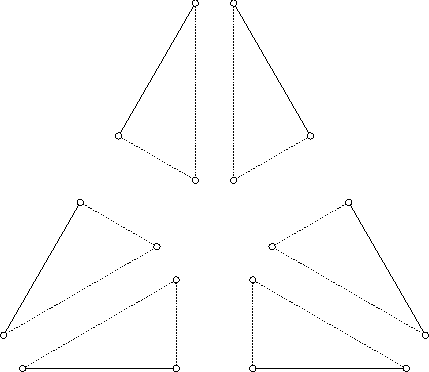
\includegraphics{figures/offset-barycentric-1.pdf}
    \caption{$\SD(c)$}
  \end{figure}
  under $\partial$, only the solid lines are not annihilated. In generality,
  \begin{align*}
    \partial \SD(c)
    &= \partial\sum_{\mathclap{\pi \in \mc S_{n+1}}} \simp[b^\pi]{n} \\
    &= \sum_{\pi \in \mc S_{n+1}} \sum_{j=0}^n \simpdel[b^\pi]{j}{n} \\
    &= \sum_{j=0}^n \sum_{\pi \in \mc S_{n+1}} \simpdel[b^\pi]{j}{n} \\
    &= \sum_{j=0}^{n-1} \sum_{\pi' \in \mc S_{n}} \simp[b^{\pi'}]{n-1} \\
    &= \SD(\partial c)
  \end{align*}
  as desired.\footnote{$\pi'$ is the permutation given by $\pi^{-1}(j_0) =
    \pi(j_0)$, where $j_0$ is the deleted vertex.}
\end{solution}
% \begin{problem}[16.21]
%   Show that $\lambda_\# \circ \SD = \msf{id}$, the identity map on $\msf
%   C_n(K)$, and therefore $\lambda_* \circ \SD_* = \msf{id}_*$, the identity map
%   on $\msf H_n(K)$.
% \end{problem}
% \begin{solution}
%   Recall the definition:
%   \[
%     \lambda_\# \sigma_i
%     =
%     \begin{cases}
%       \mb 0 & \text{if } f(\sigma_i) \text{ is not an $n$-simplex}, \\
%       \lambda(\sigma) & \text{otherwise.}
%     \end{cases}
%   \]
% \end{solution}

\begin{note}
  \color{green} I think that it's getting a little tricky here to see which
  concepts are the ``important parts.'' Maybe let's shift to trying
  \texttt{http://www.indiana.edu/~lniat/m621notessecondedition.pdf}
\end{note}

\section{The Mayer-Vietoris Theorem}
\begin{definition}[Subcomplex]
  If $K$ is a simplicial complex, a \emph{subcomplex} is a simplicial complex
  $L$ such that $L \subset K$.
\end{definition}
\begin{note}
  The thing to note here is that if we choose some simplex to be in our
  subcomplex, we must bring all its faces with us as well.
\end{note}
\begin{problem}[16.31]
  If $K$ is a finite simplicial complex, verify that the intersection of two
  subcomplexes of $K$ is a subcomplex.
\end{problem}
\begin{solution}
  Let $L, M$ be subcomplexes of $K$. Then for all $\sigma \in L \cap
  M$, $\sigma \in L,\ \sigma \in M$, hence for all faces $\sigma'
  \subset \sigma$, we have $\sigma' \in L,\ \sigma' \in M$, and thus
  $\sigma'\in L \cap M$. Hence $L \cap M$ is a simplicial complex.

  The disjointness condition follows similarly.
\end{solution}

We'll now examine cases where we have two subcomplexes $A,B$ of a
simplicial complex $K$. We want to look at relationships between
cycles in $A,B, A\cap B$, and $K$.

\begin{figure}[H]
  \centering
  \begin{subfigure}{.4\linewidth}
    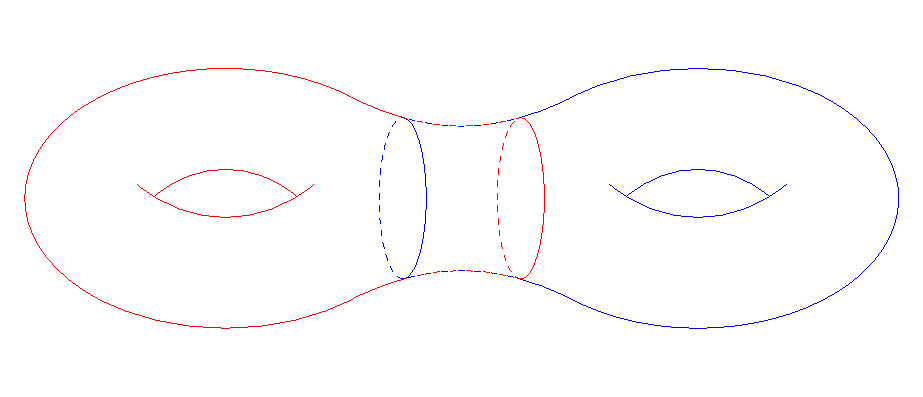
\includegraphics[width=\linewidth, keepaspectratio]{figures/mayer-vie-torus}
  \end{subfigure}
  \begin{subfigure}{.18\linewidth}
    \begin{tikzpicture}
      \draw[->] (-1,1) -- (1,1);
    \end{tikzpicture}
  \end{subfigure}
  \begin{subfigure}{.4\linewidth}
    \hspace{-.8cm}
    ~\vspace{-.5cm}
    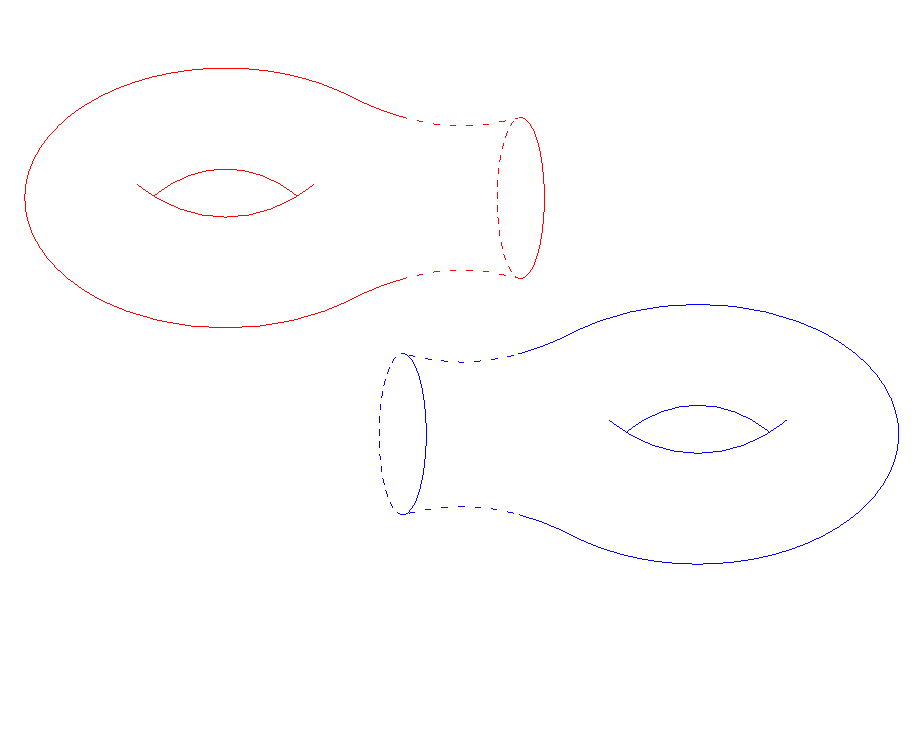
\includegraphics[width=\linewidth, keepaspectratio]{figures/mayer-vie-torus-sep}
  \end{subfigure}
  \caption{An example of such $A,B$}
\end{figure}

\begin{problem}[16.32]
  Note that a cycle in $A \cap B$ is still a cycle in $A$, $B$, and
  $K$. Then answer:
  \begin{enumerate}
  \item Can a trivial cycle in $A \cap B$ be non-trivial in $A$?
  \item Can a non-trivial cycle in $A \cap B$ be trivial in $A$?
  \item Can a non-trivial cycle in $A \cap B$ that's also
    non-trivial in $A$ and in $B$ be trivial in $K$?
  \end{enumerate}
\end{problem}
\begin{solution}
  Let $\sigma \in A \cap B$. I'll assume this is asking us to just
  consider just the inclusion map applied to $\sigma$
  \begin{enumerate}
  \item Nope. Including into $A$ won't change $\sigma$ at all.
  \item No?
  \item No?
  \end{enumerate}
\end{solution}

\begin{definition}[``Intersection'' map]
  Let $A,B$ be subcomplexes of a simplicial complex $K$. Define the
  homomorphisms $\pi_A : \msf Z_k(K) \to \msf Z_k(A)$, $\pi_B : \msf
  Z_k(K) \to \msf Z_k(B)$ as follows:
  \[
    \pi_A(\sigma) =
    \begin{cases}
      \sigma & \text{if } \sigma \in \msf Z_k(A) \\
      \mb 0 & \text{otherwise}
    \end{cases}
    \qquad\qquad
    \pi_B(\sigma) =
    \begin{cases}
      \sigma & \text{if } \sigma \in \msf Z_k(B) \\
      \mb 0 & \text{otherwise}
    \end{cases}
  \]
  Observe that the following diagram commutes, and that $\pi_A$,
  $\pi_B$ are idempotent:\footnote{Ok, technically $\dom \pi_A = \msf
    Z_k(K) \neq \msf Z_k(B)$, but you could throw an inclusion map in
    there if you so pleased.}
  \begin{figure}[H]
    \centering
    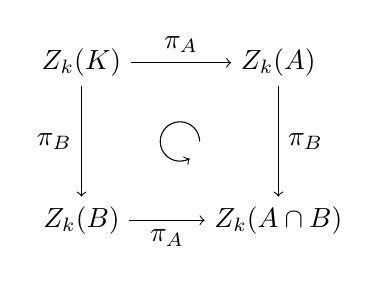
\begin{tikzpicture}
      \node (K) at (-1.25,1) {$\msf Z_k(K)$};
      \node (A) at (1.25,1) {$\msf Z_k(A)$};
      \node (B) at (-1.25,-1) {$\msf Z_k(B)$};
      \node (AcB) at (1.25,-1) {$\msf Z_k(A\cap B)$};

      \draw[->] (K) -- (A) node[midway, above] {$\pi_A$};
      \draw[->] (A) -- (AcB) node[midway, right] {$\pi_B$};
      \draw[->] (K) -- (B) node[midway, left] {$\pi_B$};
      \draw[->] (B) -- (AcB) node[midway, below] {$\pi_A$};

      \pgfmathsetmacro{\r}{.25}
      \draw[->] (\r,0) arc(0:300:\r);
    \end{tikzpicture}
    \caption{$\pi_A \circ \pi_B = \pi_B \circ \pi_A$}
  \end{figure}
\end{definition}

\begin{problem}[16.33]
  Let $K$ be a finite simplicial complex and $A$ and $B$ be
  subcomplexes such that $K=A\cup B$. If $\alpha$, $\beta$ are
  $k$-cycles in $A$ and $B$ respectively, and if $\alpha
  \sim_{\zmod{2}} \beta$ in $K$, then there is a $k$-cycle $c$ in
  $A\cap B$ such that $\alpha \sim_{\zmod{2}} c$ in $A$ and $\beta
  \sim_{\zmod{2}} c$ in $B$.
\end{problem}
\begin{solution}
  The question can be rephrased as
  \begin{leftbar}
    Let $\alpha \in \msf Z_k(A)$, and $\beta \in \msf Z_k(B)$. Suppose
    that
    \[
      [\alpha]_K = [\beta]_K.
    \]
    Then there exists $c \in \msf Z_k(A \cap B)$ such that
    \[
      [\alpha]_A = [c]_A \qquad\qquad [\beta]_B = [c]_B
    \]

    Or, show that if $\alpha - \beta = 0 \in \msf H_k(K)$, then
    $\exists c \in \msf Z_k(A \cap B)$ such that $(\alpha, \beta) =
    (c,c) \in \msf H_k(A) \oplus \msf H_k(B)$. This gives us maps
    \[
      \msf H_n(K) \xrightarrow{\delta^{k}} \msf H_k(A \cap B)
      \xrightarrow{\phi^{k}}  \msf H_k(A) \oplus \msf H_k(B)
    \]
    by
    \[
      [\alpha] = [\beta] \xmapsto{\delta^k} [c] \xmapsto{\phi^k}
      [(c,c)]
    \]
  \end{leftbar}
  Since $[\alpha]_K = [\beta]_K$, there exists $c_0 \in \msf B_k(K)$
  such that $\alpha - \beta = c_0$. By definition of $\msf B_n(K)$,
  this implies that there exists $\gamma \in \msf C_{k+1}(K)$ with
  $c_0 = \partial \gamma$.

  \textbf{Claim:} $c = \alpha + \partial \pi_A(\gamma)$ works.

  \textbf{Proof of Claim:}
  \begin{enumerate}
    \item First, we show $c$ is a $k$-cycle. Note
      \begin{align*}
        \partial c
        &= \partial \alpha + \partial^2 \pi_A(\gamma) \\
        &= \partial \alpha = \mb 0
      \end{align*}
      as desired.
    \item Now, we verify that equivalences. First, note that $c-\alpha
      = \partial \pi_A(\gamma)$, hence $[\alpha]_A = [c]_A$ trivially.
      Now,
      \begin{align*}
        c-\beta
        &= c - \alpha + \alpha - \beta & (0=\alpha - \alpha)\\
        &= (c-\alpha) + \alpha - \beta & (\text{grouping})\\
        &= \partial \pi_A(\gamma) + \alpha - \beta & (c-\alpha=\partial \pi_A(\gamma))\\
        &= \partial \pi_A(\gamma) + c_0 & (c_0 = \alpha - \beta)\\
        &= \partial \pi_A(\gamma) + \partial \gamma & (\partial \gamma = c_0)\\
        &= \partial (\pi_A\gamma + \gamma) & (\partial \text{ commutes})
      \end{align*}
      hence $c - \beta \in \msf B_k(K)$. So $[c]_B = [\beta]_B$, as
      desired.
  \end{enumerate}
\end{solution}

\begin{problem}[16.34]
  Let $K$ be a finite simplicial complex and $A$ and $B$ be
  subcomplexes such that  $K=A\cup B$. Let $z$ be a $k$-cycle in $K$.
  Then there exist $k$-chains $\alpha$ and $\beta$ in $A$ and $B$
  respectively such that:
  \begin{enumerate}[label=(\arabic*)]
    \item $z=\alpha+\beta$ and
    \item $\partial \alpha=\partial \beta$ is a $(n-1)$-cycle $c$ in
      $A\cap B$.
    \item If $z= \alpha'+\beta'$, a sum of $n$-chains in $A$ and $B$
      respectively, and $c'= \partial \alpha' = \partial \beta'$ is a
      $(n-1)$-cycle, then $c'$ is homologous to $c$ in $A \cap B$.
  \end{enumerate}
\end{problem}

\begin{solution}
  \begin{enumerate}[label=(\arabic*)]
    \item Let $\alpha = \pi_A(z)$. Then $\alpha \in \msf C_k(A)$. Now,
      taking $\beta = z - \alpha$, we see
      \begin{align*}
        \pi_A(\beta)
        &= \pi_A(z - \alpha) \\
        &= \pi_A(z - \pi_A(\alpha)) \\
        &= \pi_A(z) - \pi_A(\pi_A(z)) \\
        &= \pi_A(z) - \pi_A(z) \\
        &= \mb 0
      \end{align*}
      hence $\beta \in \msf C_k(B)$.
    \item WTS $\partial \alpha = \partial \beta \in \msf Z_{n-1}(A
      \cap B)$. Note,
      \begin{align*}
        \partial(\beta)
        &= \partial(z - \alpha) \\
        &= \partial(z) - \partial(\alpha) \\
        &= \mb 0 -\partial(\alpha) = \partial(\alpha),
      \end{align*}
      which are $(n-1)$-boundaries (and hence $(n-1)$-cycles).
      Projection onto $A \cap B$ yields the desired result.
    \item In $A \cap B$, $c$ and $c'$ are both $(n-1)$ boundaries.
      Hence, they are trivially homologous.
  \end{enumerate}
\end{solution}

\begin{problem}[16.36]
  Let $K$ be a simplicial complex and $A$ and $B$ be subcomplexes such
  that $K=A\cup B$. Construct natural homomorphisms $\phi,\psi,\delta$
  among the groups below and show that $\psi \circ \phi =0$ and
  $\delta \circ \psi = 0$.
  \begin{enumerate}
    \item $\phi: \msf H_n(A\cap B)\to \msf H_n(A)\oplus \msf H_n(B)$.
    \item $\psi: \msf H_n(A)\oplus \msf H_n(B)\to \msf H_n(K)$.
    \item $\delta: \msf H_n(K)\to \msf H_{n-1}(A\cap B)$.
  \end{enumerate}
\end{problem}
\begin{solution}
  Let
  \begin{enumerate}[label=(\arabic*)]
    \item $\phi : \msf H_n(A \cap B) \to \msf H_n(A) \oplus \msf
      H_n(B)$ be given by
      \[
        \phi(\sigma) = (\sigma, \sigma).
      \]
      That this is a well-defined homomorphism follows immediately.
    \item Let $\psi(\sigma, \tau)$ be given by
      \[
        \psi(\alpha,\beta) = \alpha - \beta.
      \]
      It is straightforward to verify this is a well-defined
      homomorphism.
    \item Let $\sigma \in \msf H_n(K)$, and take $\tau \in \msf
      Z_n(K)$ a representative of $\sigma$. Then $\exists c \in \msf
      B_n(K)$ such that
      \[
        \sigma + \tau = c.
      \]
      Then by the theorem above, there exists $\alpha \in \msf C_n(A),
      \beta \in \msf C_n(B)$
      such that
      \[
        \alpha + \beta = c.
      \]
      Further, $\partial \alpha$, $\partial \beta$ is an $(n-1)$-cycle
      $c'$ in $A \cap B$.

      Let $\delta(\sigma)$ be given by
      \[
        \delta(\sigma) = \partial(\pi_A \sigma).
      \]
      That this is a well-defined homomorphism follows, since all the
      maps included are linear.
  \end{enumerate}
  Now, we show the composition things.
  \begin{enumerate}
    \item
      \begin{align*}
        \psi \circ \phi(\alpha)
        &= \psi(\alpha, \alpha) \\
        &= \alpha - \alpha \\
        &= \mb 0
      \end{align*}
      as desired.
    \item Let $\alpha \in \msf H_n(A)$, $\beta \in \msf H_n(B)$. Then
      by the theorem above, there exists
      \begin{align*}
        \delta(\psi(\alpha, \beta))
        &= \partial (\pi_A (\alpha - \beta)) \\
        &= \partial(\alpha - \pi_A(\beta))
      \end{align*}
      \begin{figure}[H]
        \centering
        \includegraphics[width=\linewidth, keepaspectratio]{figures/two-torus-AB}
        \caption{Example of $A,B$ with $\alpha, \beta$.}
      \end{figure}
  \end{enumerate}
\end{solution}


\begin{definition}[Exact sequence]
  Given a (finite or infinite) sequence of groups and homomorphisms:
  \[
    \cdots \to G_{i-1}\stackrel{\phi_{i-1}}{\longrightarrow} G_{i}
    \stackrel{\phi_i}{\longrightarrow}G_{i+1} \to \cdots
  \]
  the sequence is \textbf{exact at $G_i$} if and only if $\im
  \phi_{i-1}=\ker \phi_{i}$. The sequence is called an \textbf{exact
    sequence} if and only if it is exact at each group (except at the
  first and last groups if they exist).
\end{definition}


\begin{problem}[16.37]
  Let $K$ be a finite simplicial complex and $A$ and $B$ be
  subcomplexes such that $K=A\cup B$. The sequence
  \[
    \dots \to \msf H_n(A\cap B) \to \msf H_n(A)\oplus \msf H_n(B) \to
    \msf H_n(K) \to \msf H_{n-1}(A\cap B) \to \dots
  \]
  using the homomorphisms $\phi,\psi,\delta$ above, is exact.
\end{problem}

\begin{enumerate}
  \item
\end{enumerate}

\begin{problem}[16.39]
  Compute the $\zmod 2$-homology groups for each complex $K$ below.
  \begin{enumerate}
    \item The bouquet of $k$ circles (the union of $k$ circles
      identified at a point).
    \item A wedge of a $2$-sphere and a circle (the two spaces are
      glued at one point).
    \item A $2$-sphere union its equatorial disk.
    \item A double solid torus.
  \end{enumerate}
\end{problem}
\begin{solution}
  \begin{enumerate}
    \item $K$ is given by $k$ triangles (together with their faces),
      with one common vertex. Hence
      \[
        \msf H_1(K) = (\zmod{2})^k \qquad\qquad \msf H_0(K) =
        (\zmod{2})^k
      \]
    \item Observe that $K = \partial \Delta^3 \cup \partial \Delta^2 /
      v_1 \sim v_2$ (where $v_1$, $v_2$ are arbitrarily chosen
      vertices from $\partial \Delta^3$, $\partial \Delta^2$
      respectively). There are just two elements of $\msf H_2(K)$:
      namely, $\mb 0$ and $A_1 + A_2 + A_3 + A_4$. Hence, $\msf H_2(K)
      \cong \zmod{2}$.

      Now, since $\partial^2 \Delta^3 = 0$, $\msf H_1(\partial^2
      \Delta^3)$ is trivial. Observe that $\msf H_1(\partial \Delta^2)
      = \zmod{2}$. Now,
    \item
    \item
  \end{enumerate}
\end{solution}


\begin{problem}[16.40]
  Compute the $\zmod{2}$-homology groups of a torus using
  Mayer-Vietoris in two different ways (with two different
  decompositions).
\end{problem}
\begin{solution}
  By Mayer-Vietoris, independent of our particular decomposition, we
  will have the following exact sequence:
  \begin{figure}[H]
    \centering
    \begin{tikzpicture}
      \pgfmathsetmacro{\xmin}{-6};
      \pgfmathsetmacro{\xmax}{6};
      \pgfmathsetmacro{\ymin}{-3};
      \pgfmathsetmacro{\ymax}{3};
      % \draw[help lines, color=gray!30, dashed] (\xmin,\ymin) grid (\xmax,\ymax);
      % \draw[->] (\xmin,0)--(\xmax,0) node[right]{$x$};
      % \draw[->] (0,\ymin)--(0,\ymax) node[above]{$y$};

      \node (cdots) at (-4,5) {$\cdots$};

      \node (3acb) at (-4, 4) {$\msf H_3(A \cap B)$};
      \node (3apb) at (0,4) {$\msf H_3(A) \oplus \msf H_3(B)$};
      \node (3k) at (4,4) {$\msf H_3(K)$};


      \node (2acb) at (-4,2) {$\msf H_2(A \cap B)$};
      \node (2apb) at (0,2) {$\msf H_2(A) \oplus \msf H_2(B)$};
      \node (2k) at (4,2) {$\msf H_2(K)$};

      \node (1acb) at (-4,0) {$\msf H_1(A \cap B)$};
      \node (1apb) at (0,0) {$\msf H_1(A) \oplus \msf H_1(B)$};
      \node (1k) at (4,0) {$\msf H_1(K)$};

      \node (0acb) at (-4,-2) {$\msf H_0(A \cap B)$};
      \node (0apb) at (0,-2) {$\msf H_0(A) \oplus \msf H_0(B)$};
      \node (0k) at (4,-2) {$\msf H_0(K)$};

      \draw[->, rounded corners=10pt] (cdots) -- ($(3acb) + (-2,1)$) -- ++(0,-1) -- (3acb);

      \draw[->] (3acb) -- (3apb) node[midway, above] {$\phi_3$};
      \draw[->] (3apb) -- (3k) node[midway, above] {$\psi_3$};
      \draw[->, rounded corners=10pt] (3k) -- ++(2,0) node[midway, above] {$\delta_3$} -- ++(0,-1) -- ($(2acb) + (-2,1)$) -- ++(0,-1) -- (2acb);

      \draw[->] (2acb) -- (2apb) node[midway, above] {$\phi_2$};
      \draw[->] (2apb) -- (2k) node[midway, above] {$\psi_2$};
      \draw[->, rounded corners=10pt] (2k) -- ++(2,0) node[midway, above] {$\delta_2$} -- ++(0,-1) -- ($(1acb) + (-2,1)$) -- ++(0,-1) -- (1acb);

      \draw[->] (1acb) -- (1apb) node[midway, above] {$\phi_1$};
      \draw[->] (1apb) -- (1k) node[midway, above] {$\psi_1$};
      \draw[->, rounded corners=10pt] (1k) -- ++(2,0) node[midway, above] {$\delta_1$} -- ++(0,-1) -- ($(0acb) + (-2,1)$) -- ++(0,-1) -- (0acb);
      \draw[->] (0acb) -- (0apb) node[midway, above] {$\phi_0$};
      \draw[->] (0apb) -- (0k) node[midway, above] {$\psi_0$};
    \end{tikzpicture}
    \caption{Mayer Vie-torus (heh)}
  \end{figure}
  Let $A,B$ be two macaroni elbow shapes, overlapping on two
  cylindrical segments:
  \begin{figure}[h]
    \centering
    \includegraphics[keepaspectratio,width=.5\linewidth,angle=270]{figures/mathematica-torus-decomp}
    \caption{Decomposition 1: $\color{green} A$ below, $\color{orange}
      B$ above}
  \end{figure}
  Note that for $k > 2$, $\TT^2$ has no $k$-cycles, and hence
  \[
    \msf H_k(A\cap B)  \cong \msf H_k(A) \oplus \msf H_k(B) \cong \msf
    H_k(\TT^2) = \set{\mb 0}.
  \]
  by exactness of the Mayer-Vietoris sequence, $\im \delta_3 = \ker
  \phi_2 = \set{\mb 0}$. Hence, $\phi_2$ is one-to-one. We will use
  this later.

  Calculating the $n=1,0$ homology groups is easy. By Theorem 16.8,
  $\msf H_0(A \cap B) \cong \zmod{2} \times \zmod{2}$, $\msf H_0(A)
  \oplus \msf H_0(B) \cong \zmod{2}\times \zmod{2}$, and $\msf
  H_0(\TT^2) \cong \zmod{2}$.

  Now, observe that each of $\msf H_2(A \cap B)$, $\msf H_2(A)$, and
  $\msf H_2(B)$ are trivial ($A$ and $B$ bound no volume). Hence
  $\delta_2$ is injective. Furthermore, since $A \cap B$ is a disjoint
  union of two cylinders, $\msf H_1(A \cap B) \cong \zmod{2} \times
  \zmod{2}$, and $\msf H_1(A) \cong \msf H_1(B) \cong \zmod{2}$. This
  gives
  \begin{figure}[H]
    \centering
    \begin{tikzpicture}
      \pgfmathsetmacro{\xmin}{-6};
      \pgfmathsetmacro{\xmax}{6};
      \pgfmathsetmacro{\ymin}{-3};
      \pgfmathsetmacro{\ymax}{3};

      \node (cdots) at (-4,5) {$\cdots$};

      \node (3acb) at (-4, 4) {$\set{\mb 0}$};
      \node (3apb) at (0,4) {$\set{\mb 0}$};
      \node (3k) at (4,4) {$\set{\mb 0}$};


      \node (2acb) at (-4,2) {$\set{\mb 0}$};
      \node (2apb) at (0,2) {$\set{\mb 0}$};
      \node (2k) at (4,2) {$\msf H_2(K)$};

      \node (1acb) at (-4,0) {$\zmod{2} \times \zmod{2}$};
      \node (1apb) at (0,0) {$\zmod{2} \times \zmod{2}$};
      \node (1k) at (4,0) {$\msf H_1(K)$};

      \node (0acb) at (-4,-2) {$\zmod{2} \times \zmod{2}$};
      \node (0apb) at (0,-2) {$\zmod{2} \times \zmod{2}$};
      \node (0k) at (4,-2) {$\zmod{2}$};

      \draw[->, rounded corners=10pt] (cdots) -- ($(3acb) + (-2,1)$) -- ++(0,-1) -- (3acb);

      \draw[->] (3acb) -- (3apb) node[midway, above] {$\phi_3$};
      \draw[->] (3apb) -- (3k) node[midway, above] {$\psi_3$};
      \draw[->, rounded corners=10pt] (3k) -- ++(2,0) node[midway, above] {$\delta_3$} -- ++(0,-1) -- ($(2acb) + (-2,1)$) -- ++(0,-1) -- (2acb);

      \draw[->] (2acb) -- (2apb) node[midway, above] {$\phi_2$};
      \draw[->] (2apb) -- (2k) node[midway, above] {$\psi_2$};
      \draw[->, rounded corners=10pt] (2k) -- ++(2,0) node[midway, above] {$\delta_2$} -- ++(0,-1) -- ($(1acb) + (-2,1)$) -- ++(0,-1) -- (1acb);

      \draw[->] (1acb) -- (1apb) node[midway, above] {$\phi_1$};
      \draw[->] (1apb) -- (1k) node[midway, above] {$\psi_1$};
      \draw[->, rounded corners=10pt] (1k) -- ++(2,0) node[midway, above] {$\delta_1$} -- ++(0,-1) -- ($(0acb) + (-2,1)$) -- ++(0,-1) -- (0acb);
      \draw[->] (0acb) -- (0apb) node[midway, above] {$\phi_0$};
      \draw[->] (0apb) -- (0k) node[midway, above] {$\psi_0$};
    \end{tikzpicture}
    \caption{Summary of results so far}
  \end{figure}
  Finally, we apply exactness. Since $\dom{\psi_2} = \set{\mb 0}$,
  $\im \psi_2 = \ker \delta_2 = \set{\mb 0}$, hence $\delta_2$ is 1-1.
  Now, note that $\ker \psi_1 = \set{(0,0), (1,1)} = \im \phi_1$.
  Hence, $\ker \phi_1 \cong \zmod{2} \cong \im \delta_2$. It follows
  that $\msf H_2(K) \cong \zmod{2}$.
  \begin{figure}[H]
    \centering
    \begin{tikzpicture}
      \pgfmathsetmacro{\xmin}{-6};
      \pgfmathsetmacro{\xmax}{6};
      \pgfmathsetmacro{\ymin}{-3};
      \pgfmathsetmacro{\ymax}{3};

      \node (cdots) at (-4,3) {$\cdots$};

      \node (2acb) at (-4,2) {$\set{\mb 0}$};
      \node (2apb) at (0,2) {$\set{\mb 0}$};
      \node (2k) at (4,2) {$\zmod{2}$};

      \node (1acb) at (-4,0) {$\zmod{2} \times \zmod{2}$};
      \node (1apb) at (0,0) {$\zmod{2} \times \zmod{2}$};
      \node (1k) at (4,0) {$\zmod{2}$};

      \node (0acb) at (-4,-2) {$\zmod{2} \times \zmod{2}$};
      \node (0apb) at (0,-2) {$\zmod{2} \times \zmod{2}$};
      \node (0k) at (4,-2) {$\zmod{2}$};

      \draw[->, rounded corners=10pt] (cdots) -- ($(2acb) + (-2,1)$) -- ++(0,-1) -- (2acb);

      \draw[->] (2acb) -- (2apb) node[midway, above] {$\phi_2$};
      \draw[->] (2apb) -- (2k) node[midway, above] {$\psi_2$};
      \draw[->, rounded corners=10pt] (2k) -- ++(2,0) node[midway, above] {$\delta_2$} -- ++(0,-1) -- ($(1acb) + (-2,1)$) -- ++(0,-1) -- (1acb);

      \draw[->] (1acb) -- (1apb) node[midway, above] {$\phi_1$};
      \draw[->] (1apb) -- (1k) node[midway, above] {$\psi_1$};
      \draw[->, rounded corners=10pt] (1k) -- ++(2,0) node[midway, above] {$\delta_1$} -- ++(0,-1) -- ($(0acb) + (-2,1)$) -- ++(0,-1) -- (0acb);
      \draw[->] (0acb) -- (0apb) node[midway, above] {$\phi_0$};
      \draw[->] (0apb) -- (0k) node[midway, above] {$\psi_0$};
    \end{tikzpicture}
    \caption{Final diagram}
  \end{figure}
  we now take the second decomposition.
  \begin{figure}[h]
    \centering
    \includegraphics[width=.5\linewidth, keepaspectratio]{figures/mathematica-torus-decomp-2}
    \caption{Second Decomposition}
  \end{figure}
  For $k > 2$, all the results remain the same. Now, note that $A \cap
  B$ is given by two concentric cylinders. Since this is still the
  disjoint union of two cylinders, for $k = 0,1,2$ the homology groups
  $H_k(A \cap B)$ and $H_k(A) \oplus H_k(B)$ remain the same. Thus, an
  identical argument to that above shows that $\msf H_2(\TT^2)$, $\msf
  H_1(\TT^2)$ are likewise identical.
\end{solution}

\begin{problem}[FS1]
  Suppose that $K$ is a triangulation of two copies of $\sS^2$,
  identified at a copy of $\sS^1$. Let $A \cong \sS^2 \cong B$. Use
  Mayer-Vietoris to compute $\msf H_n(K)$.
\end{problem}
\begin{solution}
  As before, all the $\msf H_k$ are trivial for $k > 2$. For $k=0$, we
  count the number of connected components. This yields
  \begin{itemize}
    \item $\msf H_0(K) \cong \zmod{2}$
    \item $\msf H_0(A) \oplus \msf H_0(B) \cong (\zmod{2})^2$
    \item $\msf H_0(A \cap B) \cong \zmod{2}$
  \end{itemize}
  For $k=1$,
  \begin{itemize}
    \item $\msf H_1(A\cap B) \cong \zmod{2}$
    \item $\msf H_1(A) \oplus \msf H_1(B) \cong (\zmod{2})^2$
    \item
  \end{itemize}
\end{solution}

\begin{problem}[16.41]
  Use the Mayer-Vietoris Theorem to compute $\msf H_n(M)$ for every
  compact, triangulated $2$-manifold $M$. What compact, triangulated
  $2$-manifolds are not distinguished from one another by
  $\zmod{2}$-homology? What does $\msf H_2(M)$ tell you?
\end{problem}
\begin{solution}
  Let $M$ be a compact triangulated 2-manifold, and call the
  triangulation $K$. Let $A,B$ be subcomplexes of $K$ such that $A
  \cup B = K$. Then for all $k > 2$, each of $\msf H_k(M)$, $\msf
  H_k(A)$, $\msf H_k(B)$, and $\msf H_k(A) \oplus \msf H_k(B)$ are
  isomorphic to $\set{\mb 0}$.

  Suppose $M$ can be expressed as the following connected sum:
\end{solution}


\begin{problem}[16.42]
  Let $p,q\in\ZZ$ be relatively prime. Calculate $\msf H_n(L(p,q))$,
  the homology of the lens space $L(p,q)$.
\end{problem}



%%% Local Variables:
%%% TeX-master: "../main"
%%% TeX-engine: default-shell-escape
%%% TeX-command-extra-option: -pdf
%%% End: